\documentclass[11pt,table,final,fleqn,xcolor={usenames,dvipsnames,table},handout]{beamer}
\usetheme[]{Frankfurt}


\usepackage{listings}
\usepackage{multimedia} % Movies
\usepackage{fancyvrb,relsize}
\usepackage{commath}
\usepackage{graphicx}
\usepackage{array}
\usepackage{longtable}
\usepackage{algpseudocode} 
\usepackage{multirow}
\usepackage[math]{iwona}
\usepackage{wasysym}
% \usepackage[fleqn]{amsmath}
\usepackage{amssymb}
\usepackage{siunitx}
\usepackage{tikz} % Drawing
\usepackage{pgfplots}
\usepackage{pgfplotstable}
% \usepackage{fontspec}

% Presentation settings
\rowcolors[]{1}{maincolor!20}{maincolor!10}

\newcommand{\Fo}{\ensuremath{\mathit{Fo}}}

\lstset{language=Matlab,%
    %basicstyle=\color{red},
    basicstyle=\scriptsize\ttfamily,
    breaklines=true,%
    morekeywords={matlab2tikz},
    keywordstyle=\color{blue},%
    morekeywords=[2]{1}, keywordstyle=[2]{\color{black}},
    identifierstyle=\color{black},%
    stringstyle=\color{mylilas},
    commentstyle=\color{mygreen},%
    showstringspaces=false,%without this there will be a symbol in the places where there is a space
    numbers=none,%
%     numberstyle={\tiny \color{black}},% size of the numbers
%     numbersep=-2pt, % this defines how far the numbers are from the text
%     emph=[1]{for,end,break},emphstyle=[1]\color{red}, %some words to emphasise
emph=[2]{ones,int,str2double,long,single,simplify,diff,log,atan,solve,vpa,syms,doc,int,simplify,diff,log,atan,syms,interp3,interpn,histogram,ribbon,contourf,fzero,feval,fminsearch,fsolve,fminbnd,ezplot,varargin,optimset,odeset,ode15s,plotyy,ones,linprog,cftool,optimset,lsqnonlin}, emphstyle=[2]{\color{blue}},
    backgroundcolor=\color{gray!15},frame=tlbr, framerule=0pt,
    escapeinside={(*@}{@*)}
}

% To have the navigation circles without declaring subsections
\usepackage{remreset}% tiny package containing just the \@removefromreset command
\makeatletter
\@removefromreset{subsection}{section}
\makeatother
\setcounter{subsection}{1}

% For convenient figure inclusion
\DeclareGraphicsExtensions{.pdf,.png,.jpg}
\graphicspath{ {../img/} }


% \setmainfont{Yanone Kaffeesatz}
% \setmathfont(Digits,Latin,Greek)[Numbers={Lining,Proportional}]{Gentium Plus}

% TU/e colors
\definecolor{tuered}{RGB}{247,49,49}
\definecolor{tuefuchsia}{RGB}{214,0,74}
\definecolor{tuelila}{RGB}{214,0,123}
\definecolor{tuepurple}{RGB}{173,32,173}
\definecolor{tuedblue}{RGB}{16,16,115}
\definecolor{tueblue}{RGB}{0,102,204}
\definecolor{tuelblue}{RGB}{0,162,222}
\definecolor{tueorange}{RGB}{255,154,0}
\definecolor{tueyellow}{RGB}{255,221,0}
\definecolor{tuedyellow}{RGB}{206,223,0}
\definecolor{tuegreen}{RGB}{132,210,0}
\definecolor{tuedgreen}{RGB}{0,172,130}
\definecolor{tueblue2}{RGB}{0,146,181}

% For Matlab script colors
\definecolor{mygreen}{RGB}{28,172,0} % color values Red, Green, Blue
\definecolor{mylilas}{RGB}{170,55,241}

\makeatletter
% \definecolor{beamer@blendedblue}{rgb}{0.5,0.5,0.3} % changed this
\useoutertheme{smoothbars}
\useinnertheme{circles}

%%%%%%%%%%%%%%%%%%%%%%%%%%%%%%%%%%%%%%%%%%%%%%%%%%%%%%%%%%%%%%%%%%%%%%%%%%%
\definecolor{maincolor}{named}{tuelblue}
\definecolor{textcolorfg}{named}{white}
\definecolor{tuealert}{named}{tueblue}
%%%%%%%%%%%%%%%%%%%%%%%%%%%%%%%%%%%%%%%%%%%%%%%%%%%%%%%%%%%%%%%%%%%%%%%%%%%

\setbeamercolor{normal text}{fg=black,bg=white}
\setbeamercolor{alerted text}{fg=tuealert}
\setbeamercolor{example text}{fg=tuegreen!50!black}

\setbeamercolor{background canvas}{parent=normal text,bg=white}
\setbeamercolor{background}{parent=background canvas}

\setbeamercolor{title}{bg=maincolor,fg=textcolorfg} % Presentation title colors
\setbeamercolor{structure}{fg=maincolor,bg=textcolorfg}
\setbeamercolor{section in head/foot}{fg=textcolorfg,bg=maincolor}
\setbeamercolor{palette primary}{fg=textcolorfg,bg=maincolor} % changed this

\setbeamercolor{palette primary}{fg=maincolor,bg=textcolorfg} % changed this
\setbeamercolor{palette secondary}{use=structure,fg=structure.fg!100!tueblue} % changed this
\setbeamercolor{palette tertiary}{use=structure,fg=structure.fg!100!tuered} % changed this

\setbeamertemplate{navigation symbols}{} % ( Dont use )
\setbeamercolor{navigation symbols}{use=structure,fg=structure.fg!40!bg}
\setbeamercolor{navigation symbols dimmed}{use=structure,fg=structure.fg!20!bg}

\setbeamercolor{block title}{fg=textcolorfg,bg=maincolor}
\setbeamercolor{block body}{fg=black,bg=maincolor!10}

\def\colorize<#1>{%
  \temporal<#1>{\color{tuedblue!40!gray!40}}{\color{tuealert}}{\color{black}}}
  
\setlength{\mathindent}{0pt}

\makeatother

% Colored urls
\hypersetup{colorlinks,linkcolor=,urlcolor=tueblue}

% Vector format
\renewcommand{\vec}[1]{\mathbf{#1}}

\usetikzlibrary{decorations} % Drawing
\usetikzlibrary{patterns}
\usetikzlibrary{positioning}
\usetikzlibrary{shadows}
\usetikzlibrary{calc}
\usetikzlibrary{arrows}
\usetikzlibrary{decorations}
\usetikzlibrary{plotmarks}
\usetikzlibrary{shapes}
\usetikzlibrary{shadings}
\usetikzlibrary{intersections}
% Blocks
\tikzset{block/.style={rectangle,draw=maincolor,fill=maincolor!20,text width=10em,text centered,rounded corners,minimum height=4em,thick}}
\tikzset{emphblock/.style={rectangle,draw=maincolor,text centered,rounded corners,thick,top color=maincolor!10,bottom color=maincolor!30}}
% Dots
\tikzset{dot/.style={draw=tuered,circle,thick,minimum size=1mm,inner sep=0pt,outer sep=0pt,fill=white}}
\tikzset{fdot/.style={circle,draw=black,fill=black,,inner sep=1.5pt}}
\tikzset{gdot/.style={circle,draw=black,inner sep=3pt}}
\tikzset{cross/.style={cross out, draw=black, fill=none, minimum size=2*(#1-\pgflinewidth), inner sep=0pt, outer sep=0pt}, cross/.default={4pt}}
% Graphs and lines
\tikzset{line/.style={black,>=stealth',semithick}}
\tikzset{graph/.style={smooth,samples=400,tuered,semithick}}
\tikzset{interp/.style={dot,draw=tuealert,inner sep=1.5pt,minimum size=4pt,color=tuealert,fill=none}}
\tikzset{intblock/.style={line,draw=tuefuchsia,fill=tuefuchsia!50!white,fill opacity=0.3,opacity=0.6}}
\tikzset{intdot/.style={line,dot,draw=tuefuchsia,fill=tuefuchsia,opacity=0.6}}
\tikzset{gridline/.style={lightgray,ultra thin,dashed}}


\newcolumntype{L}[1]{>{\raggedright\arraybackslash}p{#1}}
\newcolumntype{R}[1]{>{\raggedleft\arraybackslash}p{#1}}

% \pgfplotsset{
% % every axis y label/.append style={at={axis cs:14,14},rotate=0,anchor=south east}
% exery axis/.style={ylabel near ticks},
% }


\renewcommand*\familydefault{\sfdefault}  % Use sans font

% \usepackage{pgfpages}
% \pgfpagesuselayout{4 on 1}[border shrink=5mm]

\title{Numerical interpolation and integration}

\author[I.~Roghair]{\underline{Ivo~Roghair}, Martin van Sint Annaland}

\institute[SPI]{{Chemical Process Intensification,\\
  Eindhoven University of Technology}}

\date


% BEGIN PRESENTATION
\begin{document}
\lstset{language=Matlab,%
    %basicstyle=\color{red},
    basicstyle=\footnotesize\ttfamily,
    breaklines=true,%
    morekeywords={matlab2tikz},
    keywordstyle=\color{blue},%
    morekeywords=[2]{1}, keywordstyle=[2]{\color{black}},
    identifierstyle=\color{black},%
    stringstyle=\color{mylilas},
    commentstyle=\color{mygreen},%
    showstringspaces=false,%without this there will be a symbol in the places where there is a space
    numbers=none,%
%     numberstyle={\tiny \color{black}},% size of the numbers
%     numbersep=-2pt, % this defines how far the numbers are from the text
%     emph=[1]{for,end,break},emphstyle=[1]\color{red}, %some words to emphasise
    emph=[2]{ones,int,simplify,diff,log,atan,syms,doc,int,simplify,diff,log,atan,syms,interp3,interpn,histogram,ribbon,contourf,fzero,feval,fminsearch,fsolve,fminbnd,ezplot,varargin,optimset,odeset,plotyy,ones,linprog,cftool,optimset,lsqnonlin}, emphstyle=[2]{\color{blue}},
    backgroundcolor=\color{gray!15},frame=tlbr, framerule=0pt,
    escapeinside={(*@}{@*)}
}
% \lstset{language=Matlab,%
%     %basicstyle=\color{red},
%     basicstyle=\footnotesize\ttfamily,
%     breaklines=true,%
%     morekeywords={matlab2tikz},
%     keywordstyle=\color{blue},%
%     morekeywords=[2]{1}, keywordstyle=[2]{\color{black}},
%     identifierstyle=\color{black},%
%     stringstyle=\color{mylilas},
%     commentstyle=\color{mygreen},%
%     showstringspaces=false,%without this there will be a symbol in the places where there is a space
%     numbers=none,%
% %     numberstyle={\tiny \color{black}},% size of the numbers
% %     numbersep=-2pt, % this defines how far the numbers are from the text
% %     emph=[1]{for,end,break},emphstyle=[1]\color{red}, %some words to emphasise
%     emph=[2]{int,simplify,diff,log,atan,syms,interp3,interpn}, emphstyle=[2]{\color{blue}}
% }

\frame[plain]{
  \titlepage
}
\part{Numerical interpolation}
\frame{\partpage}
\section{Introduction}
\subsection*{General}
\begin{frame}[label=contents]
  \frametitle{Today's outline}
  \mode<beamer>{
    \only<1>{\tableofcontents}
  }
  \only<2>{\tableofcontents[currentsection,currentsubsection]}
\end{frame}

\begin{frame}
  \frametitle{Interpolation problem}
  \begin{definition}
  Given a set of points $x_k$, $k=0,\ldots,n$, $x_i \neq x_j$ with associated function values $f_k$, $k=0,\ldots,n$, or simply: $\{x_k,f_k\}_{k=0}^n$. The interpolation problem is defined as: find a polynomial $p_n$ such that this interpolates the values of $f_k$ on the points $x_k$:
  \[
    p_n(x_k)=f_k, \quad k=0,\ldots,n
  \]
  \end{definition}
  \pause
  \begin{theorem}
    The interpolation problem for $\{x_k,f_k\}_{k=0}^n$ has a unique solution when $x_i \neq x_j$ for $i \neq j$. Note that we cannot allow multiple function values $f_k$ for the same value of $x_k$.
  \end{theorem}
\end{frame}

\frame{
  \frametitle{What is interpolation?}
  \vfill
  \tikz{\node[emphblock,text width=\textwidth] 
    {
    Interpolation means constructing additional data points within the range of, and using, a discrete set of known data points.
    \vskip1em
    It is typically performed on a uniformly spread data set, but this is not strictly necessary for all methods
    };}
  \vfill
}
\frame{
\frametitle{Is interpolation the same as curve fitting?}
\pause
\vfill
{\begin{center} \huge NO \end{center}}
\pause
\vfill
\begin{itemize}
  \colorize<3> \item Curve-fitting requires additionally some way of computing the error between function (curve) and data
  \colorize<4> \item Curve-fitting does not strictly enforce the function to match the data exactly
  \colorize<5> \item Curve-fitting may be done on multiple datapoints at one position
  \colorize<6> \item Curve-fitting is much more expensive to do, requires optimisation
\end{itemize}
\vfill
}

\begin{frame}
  \frametitle{Why do chemical engineers need interpolation?}
  \begin{itemize}
    \colorize<1> \item Comparison of two data sets which are given at different positions
    \begin{itemize}
     \colorize<1> \item An experimental data set may have been recorded at a constant rate, but the numerical solution is computed at irregular intervals
    \end{itemize}
    \colorize<2> \item Reconstruction of field values distant of computing nodes
    \begin{itemize}
      \colorize<2> \item A CFD simulation on a regular grid containing structures that are not grid-conformant requires interpolation to the structures
    \end{itemize}
    \colorize<3> \item Calculation of a physical property at a condition between those of a lookup table
    \begin{itemize}
      \colorize<3> \item The viscosity of a substance may have been measured at 20\si{\celsius} and 30\si{\celsius}, but not at the desired 28.5\si{\celsius}
    \end{itemize}
  \end{itemize}
\end{frame}

%'exp(-x)+8*sin(x)+2*x'

\frame{
  \frametitle{General}
  Several important numerical interpolation methods are discussed today:
  \vskip2em
  \begin{itemize}
  \item Piecewise constant interpolation
  \item Linear interpolation
  \begin{itemize}
    \item Bilinear interpolation
  \end{itemize}
  \item Polynomial interpolation (Newton's method)
  \item Spline interpolation
  \end{itemize}
}

\section{Piecewise constant}
\begin{frame}
  \frametitle{Today's data set}
  \footnotesize\selectfont
  \begin{columns}
    \column{0.45\textwidth}
    Download the datafile \lstinline$interpolation-dataset.mat$, which contains multiple data sets.\vskip2em\pause
    \begin{center}
      We start with \lstinline$x1$ and \lstinline$y1$:\vskip1em
      \begin{tabular}{c|r}
	$x_k$ & $f_k$ \\ \hline
	$0$ & $1.00$ \\
	$1$ & $\frac{11}{3}=3.67$ \\
	$2$ & $\frac{8}{3}=2.67$  \\
	$3$ & $1.00$ \\
	$4$ & $\frac{5}{3}=1.67$  \\
	$5$ & $\frac{23}{3}=7.67$ \\ \hline
      \end{tabular}
    \end{center}
    \column{0.55\textwidth}
    Data set $f_n(x_n)$ represented by \tikz{\node[interp]{};} at discrete intervals $x_n\in\{0,5\}$
    \vskip1em
    \centering
    \begin{tikzpicture}[domain=-1:6]
            \draw[gridline,step=1] (0,0) grid (5,5);
      \coordinate (O) at (0,0);
      % Axes
      \draw[line,->] (-0.3,0) -- (5,0) coordinate[label = {below:$x$}] (xmax);
      \draw[line,->] (0,-0.3) -- (0,5) coordinate[label = {left:$f(x)$}] (ymax);

      % Labels
      \draw (0,0) node[below left]{$0$};
      \foreach \s in {1,...,4}
      {
        \draw (\s,0) node[below]{$\s$};
        \draw (0,\s) node[left]{$\s$};
      }

      % Title
%       \draw (2.5,5) node[above]{$f(x)=\frac{x^3}{2}-\frac{10x^2}{3}+\frac{11x}{2}+1$};

      % Plots
      \node[interp] (x0) at (0,1) {};
      \node[interp] (x1) at (1,3.667) {};
      \node[interp] (x2) at (2,2.667) {};
      \node[interp] (x3) at (3,1) {};
      \node[interp] (x4) at (4,1.667) {};
      \node (bb) at (5,5.3) {};
%       \draw [graph,domain=0:4.69] plot (\x, {0.5*\x*\x*\x-(10/3)*\x*\x+5.5*\x+1});
%       \draw [graph,opacity=0.4,dashed,domain=-0.15:4.73] plot (\x, {0.5*\x*\x*\x-(10/3)*\x*\x+5.5*\x+1});
    \end{tikzpicture}
  \end{columns}
\end{frame}

\begin{frame}
  \frametitle{Piecewise constant interpolation}
  \footnotesize\selectfont
  \begin{columns}
    \column{0.45\textwidth}
%     \begin{overlayarea}{\columnwidth}{8cm}
      \begin{itemize}
	\colorize<2> \item Nearest-neighbor interpolation in the continuous range $x\in\left[0,5\right]$
	\colorize<3> \item How to treat the point halfway (e.g. at $x=2.5$)?
% 	\hspace*{-2em}
	\begin{flalign*}
	  x \in &[0, 0.5] &\rightarrow f(x) = f(0) & \\
	  x \in &]0.5, 1.5] &\rightarrow f(x) = f(1) & \\
	  x \in &]1.5, 2.5] &\rightarrow f(x) = f(2) & \\
	  x \in &]2.5, 3.5] &\rightarrow f(x) = f(3) & \\
	  x \in &]3.5, 4.5] &\rightarrow f(x) = f(4) &
	\end{flalign*}
	\vspace*{-1em}
	\colorize<4> \item Not often used for simple problems, but e.g. for 2D (Voronoi)
      \end{itemize}
%     \end{overlayarea}
    \column{0.55\textwidth}
    Data set $f_n(x_n)$ represented by \tikz{\node[interp]{};} at discrete intervals $x_n\in\{0,5\}$
    \vskip1em
    \centering
    \begin{tikzpicture}[domain=-1:6]
            \draw[gridline,step=1] (0,0) grid (5,5);
      \coordinate (O) at (0,0);
      % Axes
      \draw[line,->] (-0.3,0) -- (5,0) coordinate[label = {below:$x$}] (xmax);
      \draw[line,->] (0,-0.3) -- (0,5) coordinate[label = {left:$f(x)$}] (ymax);

      % Labels
      \draw (0,0) node[below left]{$0$};
      \foreach \s in {1,...,4}
      {
        \draw (\s,0) node[below]{$\s$};
        \draw (0,\s) node[left]{$\s$};
      }

      % Title
%       \draw (2.5,5) node[above]{$f(x)=\frac{x^3}{2}-\frac{10x^2}{3}+\frac{11x}{2}+1$};

      % Plots
      \node[interp] (x0) at (0,1) {};
      \node[interp] (x1) at (1,3.667) {};
      \node[interp] (x2) at (2,2.667) {};
      \node[interp] (x3) at (3,1) {};
      \node[interp] (x4) at (4,1.667) {};
      \node (bb) at (5,5.3) {};
%       \draw [graph,domain=0:4.69] plot (\x, {0.5*\x*\x*\x-(10/3)*\x*\x+5.5*\x+1});
%       \draw [graph,opacity=0.4,dashed,domain=-0.15:4.73] plot (\x, {0.5*\x*\x*\x-(10/3)*\x*\x+5.5*\x+1});

      % Piecewise interpolant
      \draw<2->[interp] (0,1) -- (0.5,1);
      \draw<2->[interp] (0.5,3.667) -- (1.5,3.667);
      \draw<2->[interp] (1.5,2.667) -- (2.5,2.667);
      \draw<2->[interp] (2.5,1)     -- (3.5,1);
      \draw<2->[interp] (3.5,1.667) -- (4.5,1.667);
    \end{tikzpicture}
  \end{columns}
\end{frame}

\section{Linear}
\begin{frame}
  \frametitle{Linear interpolation}
  \footnotesize\selectfont
  \begin{columns}
    \column{0.45\textwidth}
    \begin{itemize}
      \colorize<2> \item Linear interpolation to $(x,y)$ between 2 data points $(x_2,y_2)$ and $(x_3,y_3)$:
      \colorize<3> {\[ {\color<3>{tuegreen}\frac{y-y_2}{x-x_2}}=\color<3>{tuered}\frac{y_3-y_2}{x_3-x_2} \] }
      \colorize<4> \item Reordered, and more formally: 
      \[ y = y_n + (y_{n+1} - y_n)\frac{x-x_n}{x_{n+1}-x_n} \]
    \end{itemize}
    \column{0.55\textwidth}
    Data set $f_n(x_n)$ represented by \tikz{\node[interp]{};} at discrete intervals $x_n\in\{0,5\}$
    \vskip1em
    \centering
    \begin{tikzpicture}[domain=-1:6]
            \draw[gridline,step=1] (0,0) grid (5,5);
      \coordinate (O) at (0,0);
      % Axes
      \draw[line,->] (-0.3,0) -- (5,0) coordinate[label = {below:$x$}] (xmax);
      \draw[line,->] (0,-0.3) -- (0,5) coordinate[label = {left:$f(x)$}] (ymax);

      % Labels
      \draw (0,0) node[below left]{$0$};
      \foreach \s in {1,...,4}
      {
        \draw (\s,0) node[below]{$\s$};
        \draw (0,\s) node[left]{$\s$};
      }

      % Title
%       \draw (2.5,5) node[above]{$f(x)=\frac{x^3}{2}-\frac{10x^2}{3}+\frac{11x}{2}+1$};

      % Plots
      \node[interp] (x0) at (0,1) {};
      \node[interp] (x1) at (1,3.667) {};
      \node[interp] (x2) at (2,2.667) {};
      \node[interp] (x3) at (3,1) {};
      \node[interp] (x4) at (4,1.667) {};
      \node (bb) at (5,5.3) {};
%       \draw [graph,domain=0:4.69] plot (\x, {0.5*\x*\x*\x-(10/3)*\x*\x+5.5*\x+1});
%       \draw [graph,opacity=0.4,dashed,domain=-0.15:4.73] plot (\x, {0.5*\x*\x*\x-(10/3)*\x*\x+5.5*\x+1});
      
      % Interpolant points and captions
      \draw<2->[dot,draw=none] (x2) -- node[interp,color=tuered,midway,fill=white] (xy){} (x3);
      \node<2->[anchor=north east] at (xy.west) {$(x,y)$};
      \node<2->[anchor=south west] at (x2.east) {$(x_2,y_2)$};
      \node<2->[anchor=south west] at (x3.east) {$(x_3,y_3)$};
      % Slopes between the points in colors
      \draw<3>[dot,draw=tuegreen,line width=3pt] (x2) -- (xy);
      \draw<3->[dot] (x2) -- node[interp,color=tuered,midway,fill=white] (xy){} (x3);

      % Linear interpolant
      \draw<4->[interp] (0,1) node[interp]{} -- (1,3.667) node[interp]{} -- (2,2.667) node[interp]{} -- (3,1) node[interp]{} -- (4,1.667) node[interp]{} -- (4.555,5);
      \draw<4->[interp,opacity=0.5] (4.555,5) --(4.61388,5.35);
      \draw<4->[interp,opacity=0.5] (0,1) -- (-0.1,0.108);
    \end{tikzpicture}
  \end{columns}
\end{frame}

\begin{frame}
  \frametitle{Linear interpolation}
  \begin{itemize}
    \colorize<1> \item While linear interpolation is fast, and relatively easy to program, it is not very accurate
    \colorize<2> \item At the nodes, the derivatives are discontinuous i.e. not differentiable
    \colorize<3> \item Error is proportional to the square of the distance between nodes
  \end{itemize}
\end{frame}

\begin{frame}[t,fragile]
  \frametitle{Example: Linear interpolation in Matlab}
  \footnotesize\selectfont
  Consider the data set in \lstinline$sim_exp_dataset.mat$, containing a normalized concentration and time vector for an experiment and a simulation. The simulation was performed with adaptive node distance to save computation time, thus the concentration is not known at the same times. We are not able to compare yet.
  \vfill
  \begin{tikzpicture}
    \begin{axis}[
        width=\textwidth, height=5.5cm,     % size of the image
        grid = major,
        grid style={dashed, gray!30},
        %xmode=log,log basis x=10,
        %ymode=log,log basis y=10,
        xmin=0,     % start the diagram at this x-coordinate
        xmax=200,    % end   the diagram at this x-coordinate
        ymin=0,     % start the diagram at this y-coordinate
        ymax=0.02,   % end   the diagram at this y-coordinate
        /pgfplots/xtick={0,25,...,200}, % make steps of length 5
        /pgfplots/ytick={0.005,0.01,...,0.02}, % make steps of length 5
        axis background/.style={fill=white},
        ylabel=Concentration (\si{\mol\per\cubic\meter}),
        xlabel=Time (\si{\second}),
        tick align=outside,
        legend style={draw=none,fill=none}]

      % import the correct data from a CSV file
      \addplot[draw=tuered,mark=*,mark options={fill=white},mark size=0.7pt] table [id=exp]{exp_data.txt};
      \addlegendentry{Experiment};
      \addplot[draw=tueblue,mark=triangle*,mark options={fill=white},mark size=0.7pt] table [id=sim]{sim_data.txt};
      \addlegendentry{Simulation};
      % plot the stirling-formulae
%       \addplot[domain=0:60, red, thick] {1-(365/(365-x))^(365.5-x)*e^(-x)}; 
    \end{axis} 
\end{tikzpicture}
\end{frame}

\begin{frame}[t,fragile]
  \frametitle{Example: Linear interpolation in Matlab}
  \footnotesize\selectfont
  Consider the data set in \lstinline$sim_exp_dataset.mat$, containing a normalized concentration and time vector for an experiment and a simulation. The simulation was performed with adaptive node distance to save computation time, thus the concentration is not known at the same times. We are not able to compare yet.
  \vfill
    \begin{lstlisting}
% Linear interpolation
c_sim_new = interp1(t_sim,c_sim,t_exp,'linear');
diff = abs(c_exp-c_sim_new);
% Plot the solution
subplot(2,1,1); 
plot(t_exp,c_exp,'b-x',t_exp,c_sim_new,'r-o');
subplot(2,1,2);
stem(t_exp,diff);
% Compute the L2-norm
norm(diff)
    \end{lstlisting}
\end{frame}


\begin{frame}
  \frametitle{Bi-linear interpolation}
  When a 2D field of some quantity is known, we can interpolate the solution to an arbitrary position in the 2D domain $p(x,y)$ using 4 field values $f_{00}$, $f_{10}$, $f_{01}$ and $f_{11}$.
  \begin{columns}
    \column{0.5\textwidth}
      \colorize<3> 
      \begin{align*}
	g_1 &= f_{01}\frac{x_1-x}{x_1-x_0} + f_{11}\frac{x-x_0}{x_1-x_0} \\
	    &= f_{01}\frac{x_1-x}{\Delta x} + f_{11}\frac{x-x_0}{\Delta x}
      \end{align*}
      \colorize<4> 
      \[
	g_2 = f_{00}\frac{x_1-x}{\Delta x} + f_{10}\frac{x-x_0}{\Delta x}
      \]
      \colorize<5> 
      \[
	p = g_2\frac{y_1-y}{\Delta y} + g_1\frac{y-y_0}{\Delta y}
      \]
    \column{0.5\textwidth}
      \begin{tikzpicture}[scale=2.5]
	\draw[line,-,step=1] (0,0) grid (1,1);
	\coordinate (O) at (0,0);
	\node[interp,fill=tueblue] (x0) at (0,0) {};
	\node[interp,fill=tueblue] (x1) at (1,0) {};
	\node[interp,fill=tueblue] (x2) at (1,1) {};
	\node[interp,fill=tueblue] (x3) at (0,1) {};
	\node<3->[interp,draw=tuegreen,fill=tuegreen] (g1) at (0.75,1) {};
	\node<4->[interp,draw=tuegreen,fill=tuegreen] (g2) at (0.75,0) {};
	
	\node[interp,draw=tuered,fill=tuered] (p) at (0.75,0.6) {};
	
	\node[below=1ex of x0,anchor=north east] {$f_{00}=4.0$};
	\node[below=1ex of x1,anchor=north west] {$f_{10}=6.0$};
	\node[above=1ex of x2,anchor=south west] {$f_{11}=1.0$};
	\node[above=1ex of x3,anchor=south east] {$f_{01}=8.0$};
	\node[right=-0.3ex of p] {$p$};
	\node<3->[above=1ex of g1] {$g_1$};
	\node<4->[below=1ex of g2] {$g_2$};
	\draw<2>[line,dashed,gray] (x0)--(p);
	\draw<2>[line,dashed,gray] (x1)--(p);
	\draw<2>[line,dashed,gray] (x2)--(p);
	\draw<2>[line,dashed,gray] (x3)--(p);
	\draw<5->[line,-,dashed,gray] (g1)--(g2);
	
	\draw[line,stealth'-stealth'] ($(x0)+(0,0.1)$) -- node[midway,above]{$\Delta x$}($(x1)+(0,0.1)$);
	\draw[line,stealth'-stealth'] ($(x0)+(0.1,0)$) -- node[midway,right]{$\Delta y$}($(x3)+(0.1,0)$);
      \end{tikzpicture}
  \end{columns}
  \onslide<6>{ \vskip1em
  \begin{itemize}
    \item The order of interpolation ($x$ or $y$ direction first) does not matter; the results are equal
  \end{itemize}
  }
\end{frame}

\begin{frame}
  \frametitle{Higher-dimensional field interpolation in Matlab}
  2D or higher-dimensional fields of data can be interpolated in Matlab using the \lstinline$interp2$, \lstinline$interp3$ or even \lstinline$interpn$ functions, the method can be adjusted:
  \vskip1em
  \begin{columns}
    \column{0.33\textwidth}
      \centering
      \lstinline$'nearest'$
      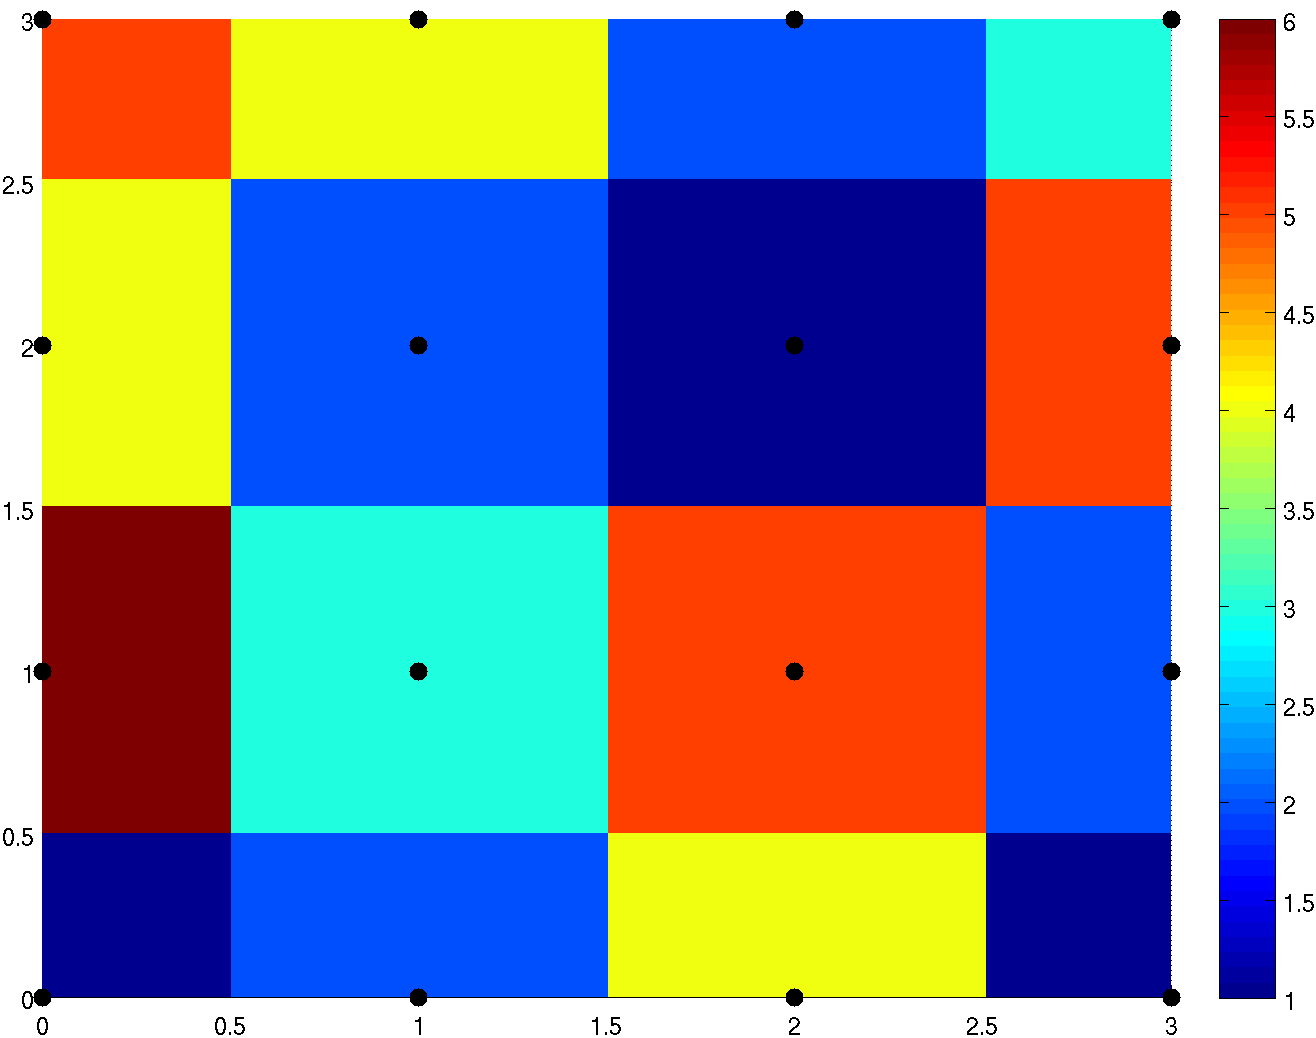
\includegraphics[width=\columnwidth]{Nearest2DInterpolExample.png}
    \column{0.33\textwidth}
      \centering
      \lstinline$'linear'$
      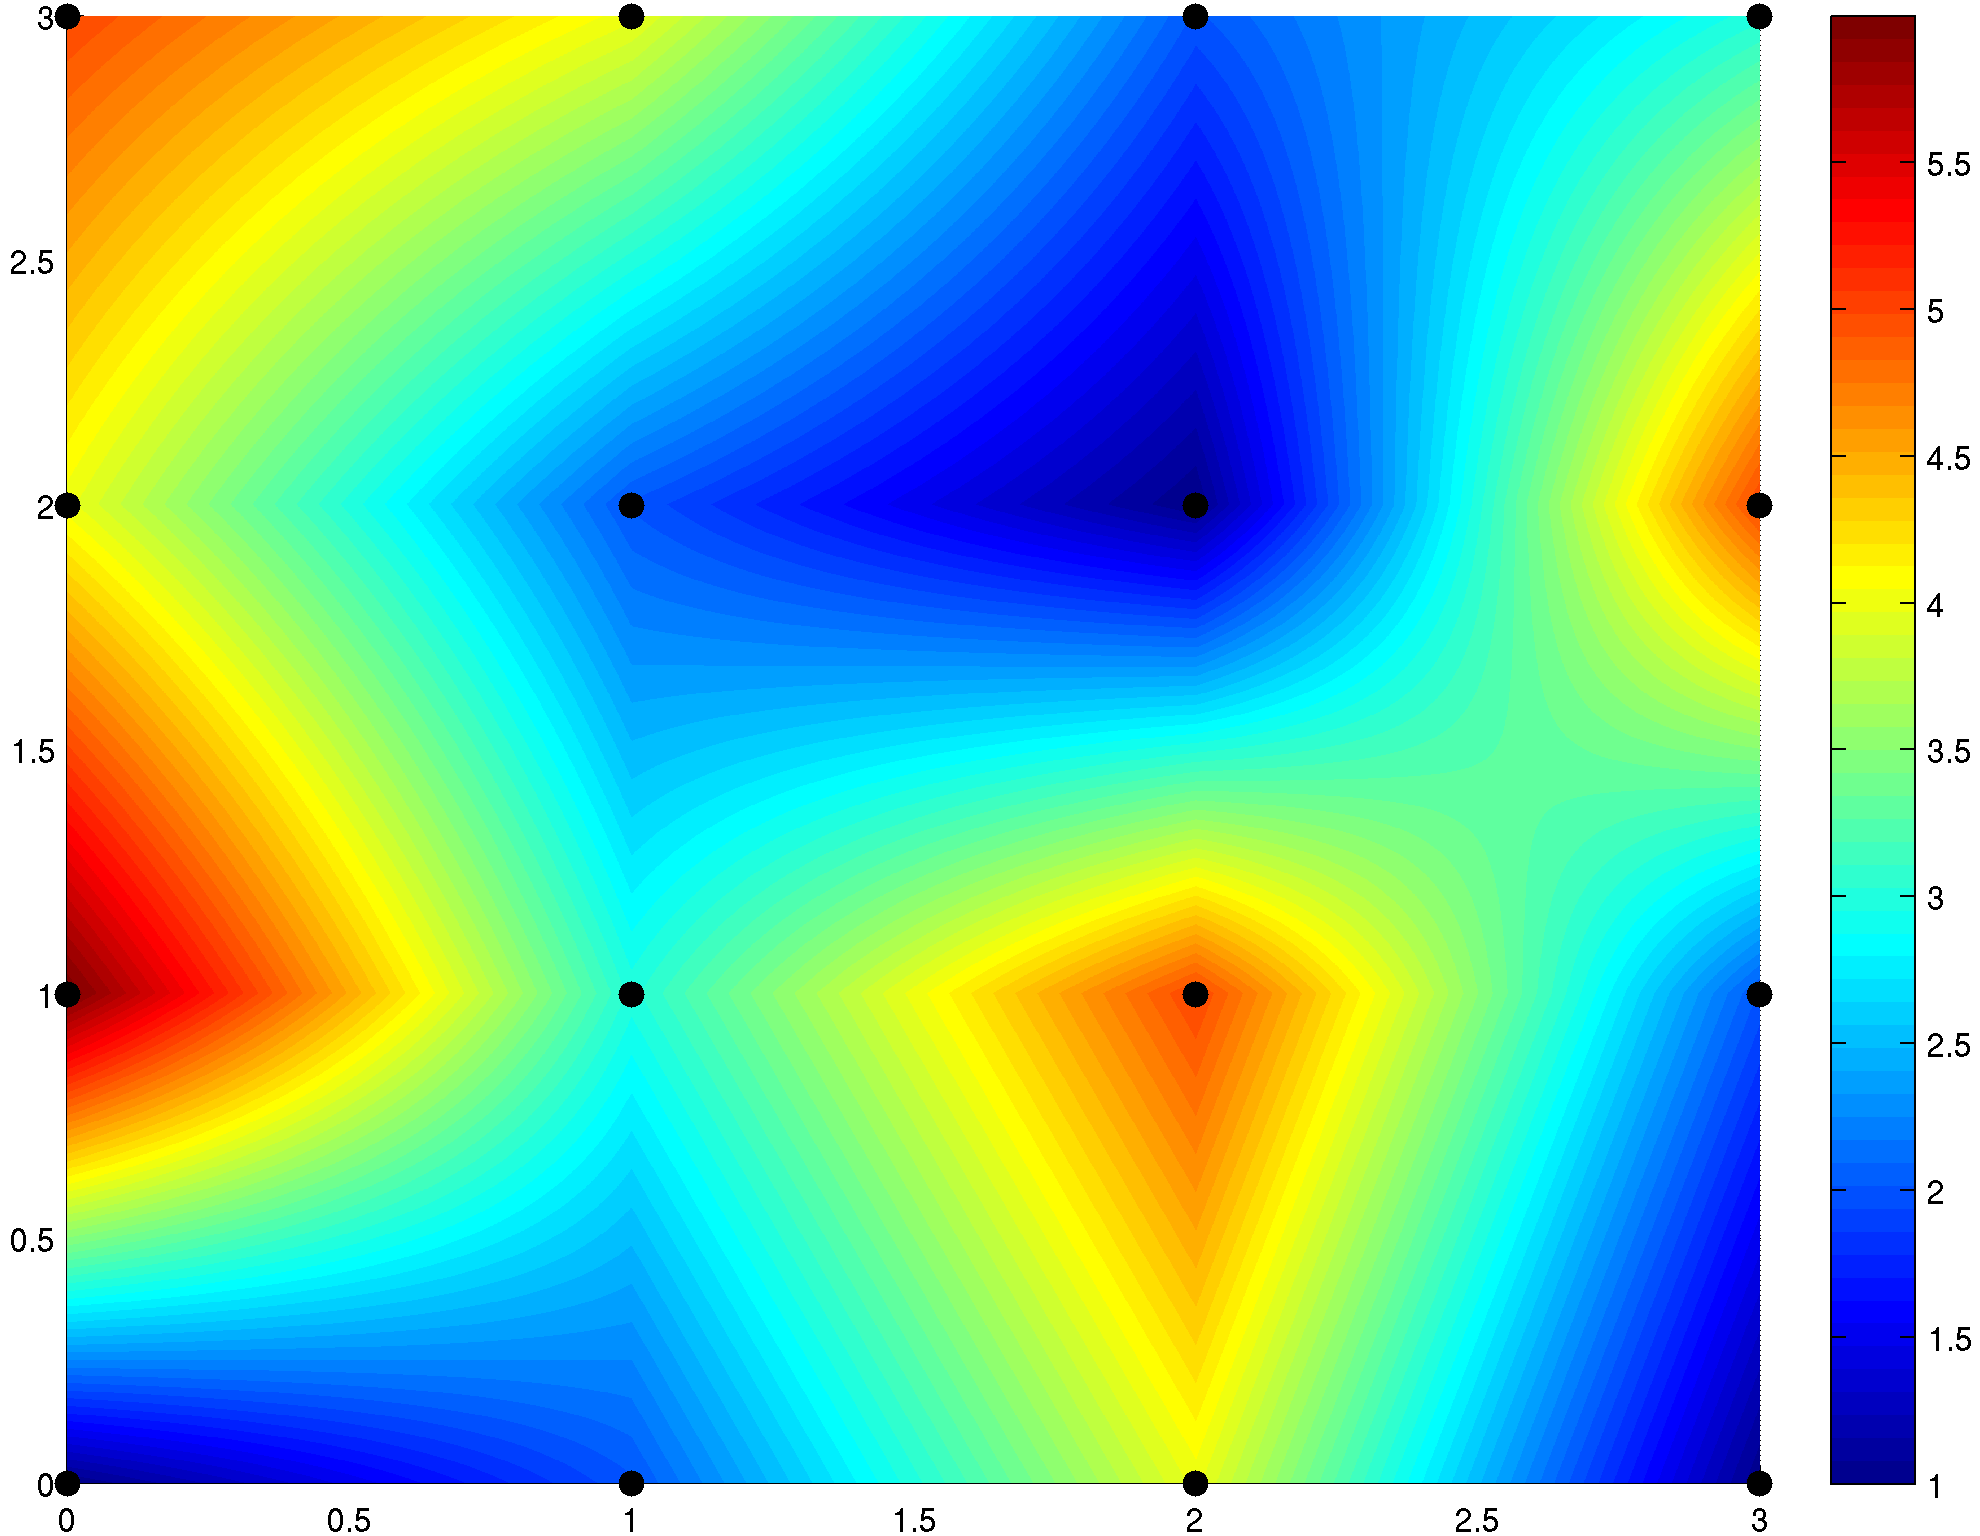
\includegraphics[width=\columnwidth]{BilinearInterpolExample.png}
    \column{0.33\textwidth}
      \centering
      \lstinline$'cubic'$
      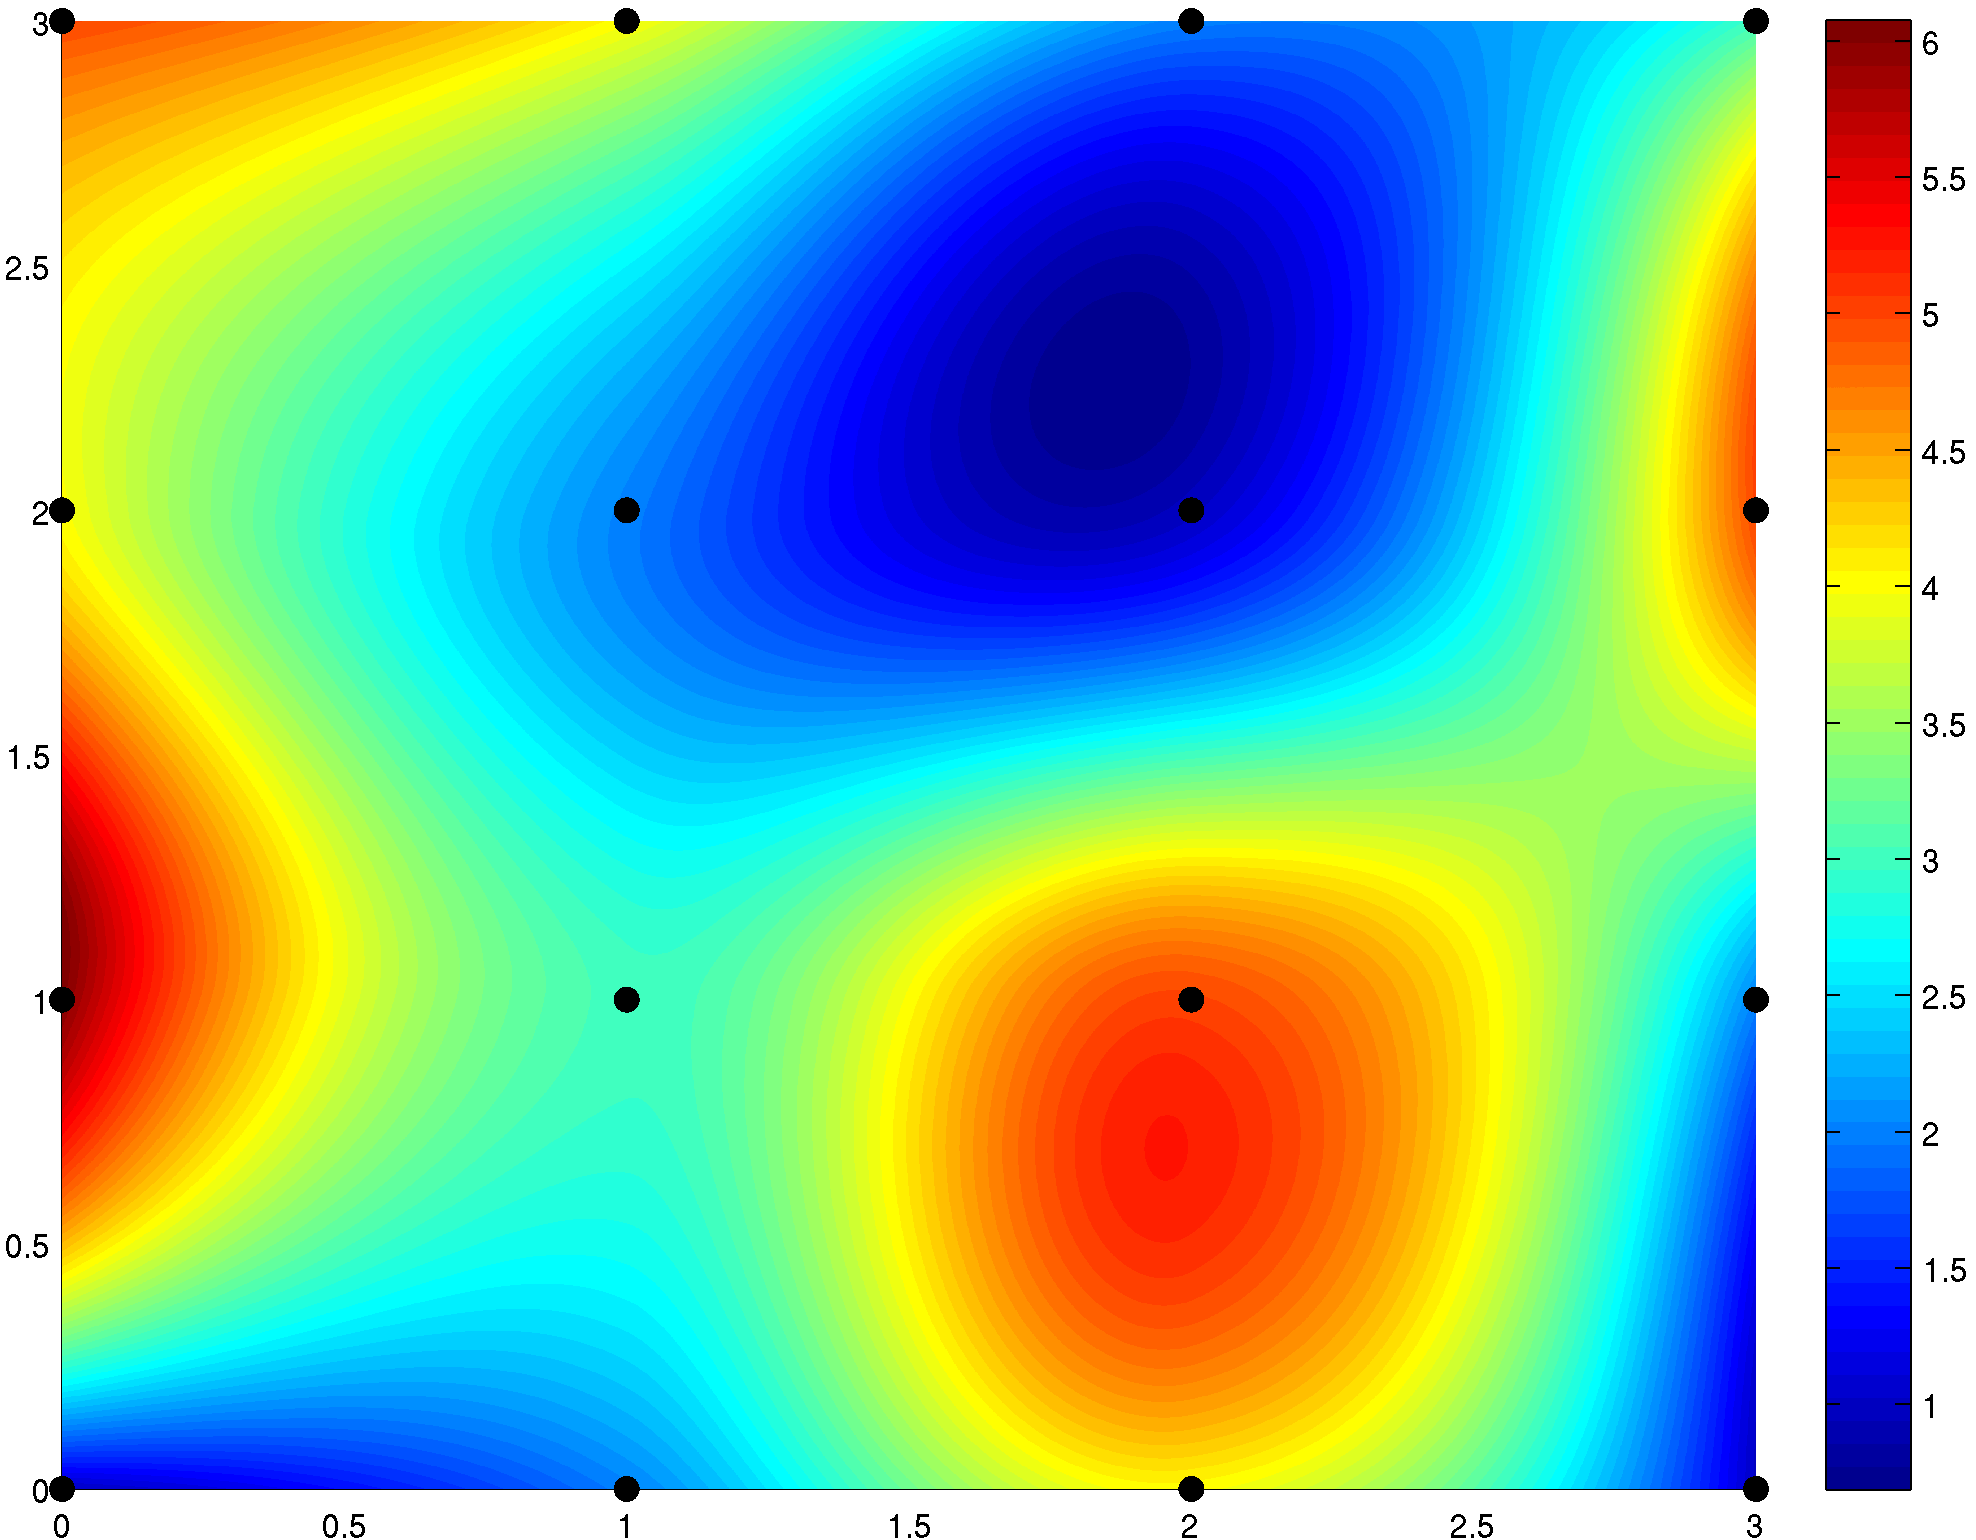
\includegraphics[width=\columnwidth]{BicubicInterpolationExample.png}
  \end{columns}
  \vskip1em
  \begin{itemize}
    \item Similar to 1D linear interpolation, the derivatives are discontinuous on the grid nodes
    \item Also consider tri-linear interpolation (for 3D fields), or bicubic interpolation (2D, but third order)
  \end{itemize}
\end{frame}

\begin{frame}
  \frametitle{A practical example}
  Field interpolation is used in e.g. CFD simulations, e.g. a fluidized bed simulation using a \emph{discrete particle model}, where particles are found in between the grid nodes used for velocity computation.
  \centering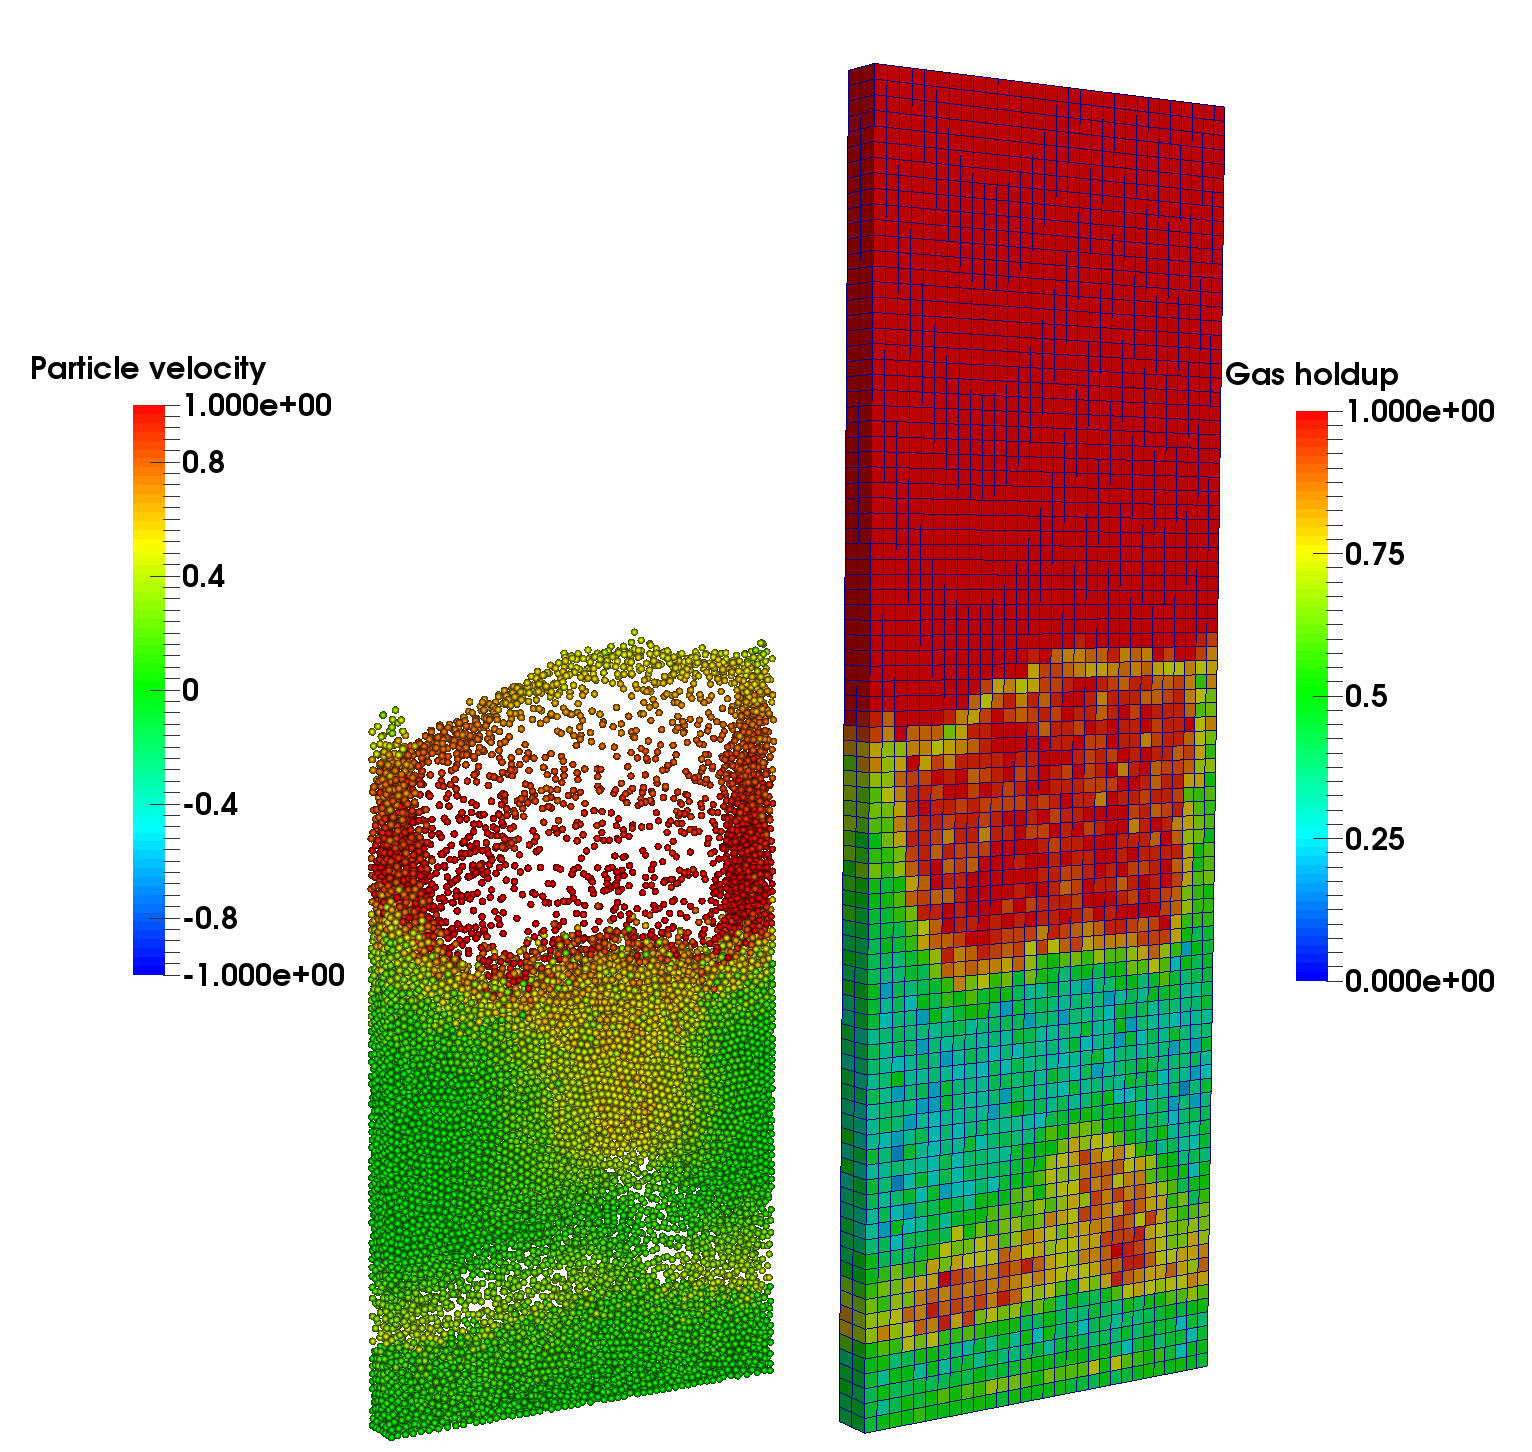
\includegraphics[width=0.6\textwidth]{fluidbed}
\end{frame}

\section{Polynomial}
\begin{frame}
  \frametitle{Polynomial interpolation}
  The examples that we have seen, are simplified forms of \emph{Newton polynomials}. We can interpolate our data with a polynomial of degree $n$:
  
  \vskip2em
  \[
    p_n(x) = a_n x^n + a_{n-1}x^{n-1} + \ldots + a_2x^2 + a_1 x + a_0
  \]

\end{frame}

\begin{frame}[fragile]
  \frametitle{Polynomial interpolation via Vandermonde matrix}
  \footnotesize\selectfont
  \rowcolors[]{50}{white}{white}
  Consider the data points $(x_1,y_1),\, (x_2,y_2),\, \ldots,\,(x_m,y_m)$, the Vandermonde matrix $V$, coefficient vector $a$ and function value vector $y$: \vskip1em
  $V_{m,n} =
 \begin{pmatrix}
  x_1^0 & x_1^1 & x_1^2 & \cdots & x_1^{n-1} \\
  x_2^0 & x_2^1 & x_2^2 & \cdots & x_2^{n-1} \\
  \vdots  & \vdots & \vdots & \ddots & \vdots  \\
  x_m^0 & x_m^1 & x_m^2 & \cdots & x_m^{n-1}
 \end{pmatrix} \quad  
 a=
 \begin{pmatrix}
   a_0 \\
   a_1 \\
   \vdots\\
   a_{n-1}
 \end{pmatrix} \quad
 y=
 \begin{pmatrix}
   y_1 \\
   y_2 \\
   \vdots\\
   y_m
 \end{pmatrix}
$\vskip1em
The coefficients of a polynomial through the data points can be obtained by solving the linear system $Va=y$.
\pause
\begin{columns}
  \column{0.5\textwidth}
    \begin{lstlisting}
    >> x = [0 1 2];
    >> y = [1.0000; 3.6667; 2.6667];
    >> V = vander(x);
    >> a = V\y
    a =
       -1.8333
        4.5000
        1.0000
    \end{lstlisting}
  \column{0.5\textwidth}
  \pause
  So we found the equation:
  \[
    p_2(x) = -1.8333 x^2 + 4.5x - 1
  \]
  \pause
  \tikz{\node[emphblock,text width=\columnwidth] {These Vandermonde-systems are often \emph{ill-conditioned}, so we need another, more stable, method!
};}
\end{columns}
\end{frame}

\begin{frame}
  \frametitle{Construction of Newton polynomials}
  \footnotesize\selectfont
  Formally, the polynomials $p_n(x)$ are described using prefactors $f[x_0,\ldots,x_k]$ and polynomial terms $w_m(x)$:
  \[
    p_n(x) = \sum_{k=0}^n f[x_0,\ldots,x_k] w_k(x)
  \]
  \pause
  The polynomial terms are computed via:
  \begin{align*}
    &w_0(x) = 1, \ w_1(x)=(x-x_0), \ w_2(x)=(x-x_0)\cdot(x-x_1), \\
    &w_m(x)=(x-x_0)\cdot(x-x_1)\cdots(x-x_{m-1}) = w_{m-1}\cdot(x-x_{m-1})\\
    &w_m(x) = \prod_{j=0}^{m-1} (x-x_j), \qquad m=0,\ldots,n
  \end{align*}
  \pause
  The prefactors are \emph{forward divided differences}, which can be computed as:
    \[
      f[x_{x-k},\ldots,x_r] \equiv \frac{f[x_{r-k+1},\ldots,x_r]-f[x_{r-k},\ldots,x_{r-1}]}{x_r-x_{r-k}} 
    \]
\end{frame}

% 
%       \begin{align*}
% 	p_n(x)                &= \sum_{k=0}^n f[x_0,\ldots,x_k] w_k(x) \\
% 	w_m(x)                &= \prod_{j=0}^{m-1} (x-x_j) \\
% 	f[x_{x-k},\ldots,x_r] &\equiv \frac{f[x_{r-k+1},\ldots,x_r]-f[x_{r-k},\ldots,x_{r-1}]}{x_r-x_{r-k}} 
%       \end{align*}

\begin{frame}
  \frametitle{Construction of Newton polynomials: example}
  \footnotesize\selectfont
  \rowcolors[]{1}{maincolor!20}{maincolor!10}
  \begin{columns}[T]
    \begin{column}{0.2\textwidth}
    \centering Sample data
      \begin{longtable}{c|r}
	$x_k$ & $f_k$ \\ \hline
	$0$ & $1.00$ \\
	$1$ & $\frac{11}{3}=3.67$ \\
	$2$ & $\frac{8}{3}=2.67$ 
      \end{longtable}
    \end{column}
    \hfill
    \begin{column}{0.8\textwidth}
      \begin{tikzpicture}[myNode/.style={rectangle,draw=maincolor,fill=maincolor!20,text centered,rounded corners,thick,minimum height=2em}]
	\node[myNode] (a) {${\scriptstyle p_n(x)= \sum_{k=0}^n f[x_0,\ldots,x_k] w_k(x)}$};
	\node[myNode,below left=1.2cm of a.south west,anchor=center] (c) {${\scriptstyle f[x_{x-k},\ldots,x_r] \equiv \frac{f[x_{r-k+1},\ldots,x_r]-f[x_{r-k},\ldots,x_{r-1}]}{x_r-x_{r-k}}}$};
	\node[myNode,below right=1.2cm of a.south east,anchor=center] (b) {${\scriptstyle w_m(x) = \prod_{j=0}^{m-1} (x-x_j)}$};
	\draw[->,>=stealth] (c.north) -> (a.south west);
	\draw[->,>=stealth] (b.north) -> (a.south east);
      \end{tikzpicture}
    \end{column}
  \end{columns}
    \onslide<2->{
      \begin{longtable}{c|ccc}
	$x_k$ & $f_k$ & & \\ \hline 
	\color<2>{tuered} $x_0$ & \color<2>{tuered} $f[x_0]=f_0$ & & \onslide<3->{\\
	\color<3>{tuered} $x_1$ & \color<3>{tuered} $f[x_1]=f_1$ & \color<3>{tuered} $f[x_0,x_1]=\frac{f_1-f_0}{x_1-x_0}$& \onslide<4->{\\
	\color<4>{tuered} $x_2$ & \color<4>{tuered} $f[x_2]=f_2$ & \color<4>{tuered} $f[x_1,x_2]=\frac{f_2-f_1}{x_2-x_1}$& \color<4>{tuered} $f[x_0,x_1,x_2] = \frac{f[x_1,x_2]-f[x_0,x_1]}{x_2-x_0}$ }}
      \end{longtable}}
  \onslide<2->{
    \begin{longtable}{c|lll}
      $x_k$ & $f_k$ & & \\ \hline
      \color<2>{tuered} $0$ & \color<2>{tuered} $1$ & & \onslide<3->{\\
      \color<3>{tuered} $1$ & \color<3>{tuered} $3.67$ & \color<3>{tuered} $\frac{\frac{11}{3}-1}{1-0}=\frac{8}{3}$& \onslide<4>{\\
      \color<4>{tuered} $2$ & \color<4>{tuered} $2.67$ & \color<4>{tuered} $\frac{\frac{8}{3}-\frac{11}{3}}{2-1}=\frac{-1}{1}=-1$& \color<4>{tuered} $\frac{(-1)-\frac{8}{3}}{2-0}=-\frac{11}{6}$ }}
    \end{longtable}
  }
\end{frame}

\begin{frame}
  \frametitle{Construction of Newton polynomials: example}
  \footnotesize\selectfont
  \rowcolors[]{1}{maincolor!20}{maincolor!10}
  \begin{columns}[T]
    \begin{column}{0.2\textwidth}
    \centering Sample data
      \begin{longtable}{c|r}
	$x_k$ & $f_k$ \\ \hline
	{\color<4->{tuedyellow}$0$} & $1.00$ \\
	{\color<4->{tuepurple}$1$} & $\frac{11}{3}=3.67$ \\
	$2$ & $\frac{8}{3}=2.67$ 
      \end{longtable}
    \end{column}
    \hfill
    \begin{column}{0.8\textwidth}
      \begin{tikzpicture}[myNode/.style={rectangle,draw=maincolor,fill=maincolor!20,text centered,rounded corners,thick,minimum height=2em}]
	\node[myNode] (a) {${\scriptstyle p_n(x)= \sum_{k=0}^n f[x_0,\ldots,x_k] w_k(x)}$};
	\node[myNode,below left=1.2cm of a.south west,anchor=center] (c) {${\scriptstyle f[x_{x-k},\ldots,x_r] \equiv \frac{f[x_{r-k+1},\ldots,x_r]-f[x_{r-k},\ldots,x_{r-1}]}{x_r-x_{r-k}}}$};
	\node[myNode,below right=1.2cm of a.south east,anchor=center] (b) {${\scriptstyle w_m(x) = \prod_{j=0}^{m-1} (x-x_j)}$};
	\draw[->,>=stealth] (c.north) -> (a.south west);
	\draw[->,>=stealth] (b.north) -> (a.south east);
      \end{tikzpicture}
    \end{column}
  \end{columns}
  \pause
  \begin{longtable}{c|lll}
    $x_k$ & $f_k$                    & & \\ \hline
      $0$ & \color{tuered} $1$     & & \\
      $1$ &                  $3.67$ & $\frac{\frac{11}{3}-1}{1-0}=\color{tuered} \frac{8}{3}$& \\
      $2$ &                  $2.67$ & $\frac{\frac{8}{3}-\frac{11}{3}}{2-1}=\frac{-1}{1}=-1$   & $\frac{(-1)-\frac{8}{3}}{2-0}=\color{tuered}-\frac{11}{6}$ 
  \end{longtable}
  \onslide<3->{
    \begin{align*}
	p_2(x) &= {\color{tuered}1}\cdot w_m(0) + {\color{tuered}\frac{8}{3}}\cdot w_m(1) + \left({\color{tuered}-\frac{11}{6}}\right)\cdot w_m(2)   \\
	\onslide<4->{&= {\color{tuered}1}\cdot 1 + {\color{tuered}\frac{8}{3}}\cdot (x-{\color{tuedyellow}0}) + \left({\color{tuered}-\frac{11}{6}}\right)\cdot (x-{\color{tuedyellow}0})(x-{\color{tuepurple}1}) \onslide<5>{= \color{tuealert}-\frac{11}{6}x^2+4\frac{1}{2}x+1}}
    \end{align*}
  }
\end{frame}


\begin{frame}
  \frametitle{Construction of Newton polynomials: example}
  For each three points, a new polynomial interpolant can be derived:
  \begin{columns}
    \column{0.45\textwidth}
      \colorize<2>\color<2->{tuered}    \[ p_2(x) = -\frac{11}{6}x^2+4\frac{1}{2}x+1 \]
      \colorize<3>\color<3->{tuelila}   \[ p_2(x) = 4-\frac{x^2}{3} \]
      \colorize<4>\color<4->{tuelblue}  \[ p_2(x) = \frac{7x^2}{6}-7\frac{1}{2}x+13 \]
      \colorize<5>\color<5->{tuedyellow} \[ p_2(x) = \frac{8}{3}x^2-18x+31 \]
    \column{0.55\textwidth}
    \centering
    \begin{tikzpicture}[domain=-1:6]
            \draw[gridline,step=1] (0,0) grid (5,5);
      \coordinate (O) at (0,0);
      % Axes
      \draw[line,->] (-0.3,0) -- (5,0) coordinate[label = {below:$x$}] (xmax);
      \draw[line,->] (0,-0.3) -- (0,5) coordinate[label = {left:$f(x)$}] (ymax);

      % Labels
      \draw (0,0) node[below left]{$0$};
      \foreach \s in {1,...,4}
      {
        \draw (\s,0) node[below]{$\s$};
        \draw (0,\s) node[left]{$\s$};
      }

      % Title
%       \draw (2.5,5) node[above]{$f(x)=\frac{x^3}{2}-\frac{10x^2}{3}+\frac{11x}{2}+1$};

      % Plots
      \node[interp] (x0) at (0,1) {};
      \node[interp] (x1) at (1,3.667) {};
      \node[interp] (x2) at (2,2.667) {};
      \node[interp] (x3) at (3,1) {};
      \node[interp] (x4) at (4,1.667) {};
      \node (bb) at (5,5.3) {};
%       \draw [graph,domain=0:4.69] plot (\x, {0.5*\x*\x*\x-(10/3)*\x*\x+5.5*\x+1});
%       \draw [graph,opacity=0.4,dashed,domain=-0.15:4.73] plot (\x, {0.5*\x*\x*\x-(10/3)*\x*\x+5.5*\x+1});

      % Polynomial interpolant
      \draw<2-> [graph,domain=0:2,draw=tuered,opacity=0.7] plot (\x, {-(11/6)*\x*\x+(4.5)*\x+1});
      \draw<3-> [graph,domain=1:3,draw,tuelila,opacity=0.7] plot (\x, {(-1/3)*\x*\x+4});
      \draw<4-> [graph,domain=2:4,draw=tuelblue,opacity=0.7] plot (\x, {(7/6)*\x*\x-7.5*\x + 13});
      \draw<5-> [graph,domain=3:4.7,draw=tuedyellow,opacity=0.7] plot (\x, {(8/3)*\x*\x-18*\x+31});
      \draw<6> [graph,domain=0:4.69,draw=tuedgreen,opacity=0.5] plot (\x, {0.5*\x*\x*\x-(10/3)*\x*\x+5.5*\x+1});
    \end{tikzpicture}
    \onslide<6>{
      \[
	\color{tuedgreen} f(x)=\frac{x^3}{2}-\frac{10x^2}{3}+\frac{11x}{2}+1
      \]
    }
    \vfill
  \end{columns}
\end{frame}

\begin{frame}[fragile]
  \frametitle{Polynomial fitting in Matlab: example}
  \rowcolors[]{1}{maincolor!20}{maincolor!10}
  \footnotesize\selectfont
     \begin{columns}
    \column{0.45\textwidth}
    Develop the {\color<5->{tuered}$p_2(x)$}, {\color<6->{tuedgreen}$p_3(x)$} and {\color<7>{tuelblue}$p_4(x)$} from the following data set (example data \lstinline$x2$ and \lstinline$y2$): 
    \vspace*{-1ex}
    \begin{center}
      \begin{tabular}{c|r}
	$x_k$ & $y_k$ \\ \hline
	$-1.0$ & $2.8677$ \\
	$-0.5$ & $7.7530$ \\
	$0.0$ & $22.0000$  \\
	$0.5$ & $65.7863$ \\
	$1.0$ & $208.6744$  \\ \hline
      \end{tabular}
    \end{center}
    \column{0.55\textwidth}
    \centering
    \begin{tikzpicture}[domain=-1:1,xscale=2,yscale=0.01]
      \draw[gridline,step=50] (-1,0) grid (1,250);
      \coordinate (O) at (0,0);
      % Axes
      \draw[line,->] (-1,0) -- (1,0) coordinate[label = {right:$x$}] (xmax);
      \draw[line,->] (0,0) -- (0,250) coordinate[label = {above:$y$}] (ymax);

      % Labels
%       \draw (0,0) node[below left]{$0$};
      \foreach \s in {-1,-0.5,...,1}
      {
        \draw (\s,0) node[below]{$\s$};
      }
      \foreach \s in {50,100,...,250}
      {
        \draw (0,\s) node[left]{$\s$};
      }

      % Title
%       \draw (2.5,5) node[above]{$f(x)=\frac{x^3}{2}-\frac{10x^2}{3}+\frac{11x}{2}+1$};

      % Plots
       \node[interp] (x0) at (-1,2.8677) {};
       \node[interp] (x1) at (-0.5,7.753) {};
       \node[interp] (x2) at ( 0.0,22.00) {};
       \node[interp] (x3) at ( 0.5,65.7863) {};
       \node[interp] (x4) at ( 1.0,208.6744) {};
       
       \draw<5-> [graph,draw=tuered,opacity=0.7,domain=-1:1] plot (\x, {87.2986*\x*\x+93.9293*\x+17.7670});
       \draw<6-> [graph,draw=tuedgreen,opacity=0.7,domain=-1:1] plot (\x, {59.8267*\x*\x*\x+87.2986*\x*\x+43.0766*\x+17.7670});
       \draw<7> [graph,draw=tuelblue,opacity=0.7,domain=-1:1] plot (\x, {32.9234*\x*\x*\x*\x+59.8267*\x*\x*\x+50.8477*\x*\x+43.0766*\x+22.0000});
    \end{tikzpicture}
  \end{columns}
  \pause \vskip1ex
  We use the built-in \lstinline$polyfit(x,y,n)$ and \lstinline$polyval(p,x)$ functions: \pause
  \begin{lstlisting}
    x_cont = linspace(-1,1,1001);
    p2 = polyfit(x2,y2,2);
    p3 = polyfit(x2,y2,3);
    p4 = polyfit(x2,y2,4);
    \end{lstlisting} \pause \vskip-1em
    \begin{lstlisting}
    y_cont2 = polyval(p2,x_cont);
    y_cont3 = polyval(p3,x_cont);
    y_cont4 = polyval(p4,x_cont);
    plot(x2,y2,'o',x_cont,y_cont2,x_cont,y_cont3,x_cont,y_cont4)  \end{lstlisting}
\end{frame}



\begin{frame}[fragile]
  \frametitle{Exercise}
  \rowcolors[]{1}{maincolor!20}{maincolor!10}
  \footnotesize\selectfont
  Develop the {\color<4->{tuered}$p_4(x)$} and {\color<5>{tueorange}$p_{10}(x)$} interpolants from the following data sets: 
     \begin{columns}
    \column{0.55\textwidth}
    \vspace*{-1em}
\[
f(x)=\frac{1}{x^2+\frac{1}{25}} \qquad x \in [-1,1]
\]
     \begin{lstlisting}
x3a = linspace(-1 , 1 , 5);
x3b = linspace(-1 , 1 , 11);
y3a = 1 ./ (x3a.^2 + (1/25));
y3b = 1 ./ (x3b.^2 + (1/25));
    \end{lstlisting}
    \column{0.45\textwidth}
    \centering
    \begin{tikzpicture}[domain=-1:1,xscale=2,yscale=0.1]
      \clip(-1.2,-10) rectangle (1.2,35);
      \draw[gridline,step=5] (-1,0) grid (1,30);
      \coordinate (O) at (0,0);
      % Axes
      \draw[line,->] (-1,0) -- (1,0) coordinate[label = {right:$x$}] (xmax);
      \draw[line,->] (0,0) -- (0,30) coordinate[label = {above:$y$}] (ymax);

      % Labels
%       \draw (0,0) node[below left]{$0$};
      \foreach \s in {-1,-0.5,...,1}
      {
        \draw (\s,0) node[below]{$\s$};
      }
      \foreach \s in {5,10,...,30}
      {
        \draw (-1,\s) node[left]{$\s$};
      }
   
      \node[interp] (x0a) at (-1.0000 , 0.9615) {};
      \node[interp] (x1a) at (-0.5000 ,   3.4483) {};
      \node[interp] (x2a) at ( 0 , 25.0000) {};
      \node[interp] (x3a) at ( 0.5000  ,  3.4483) {};
      \node[interp] (x4a) at ( 1.0000,    0.9615) {};
      \node[dot] (x0b) at (-1.0000,    0.9615) {};
      \node[dot] (x1b) at (-0.8000,    1.4706) {};
      \node[dot] (x2b) at (-0.6000,    2.5000) {};
      \node[dot] (x3b) at (-0.4000,    5.0000) {};
      \node[dot] (x4b) at (-0.2000,   12.5000) {};
      \node[dot] (x5b) at ( 0.0000,   25.0000) {};
      \node[dot] (x6b) at ( 0.2000,   12.5000) {};
      \node[dot] (x7b) at ( 0.4000,    5.0000) {};
      \node[dot] (x8b) at ( 0.6000,    2.5000) {};
      \node[dot] (x9b) at ( 0.8000,   1.4706) {};
      \node[dot] (x10b) at (1.0000,    0.9615) {};

      \draw<3-> [graph,draw=tuelblue,opacity=0.7,domain=-1:1] plot (\x, {1/(\x*\x+(1/25))});
      \draw<4-> [graph,draw=tuered,opacity=0.7,domain=-1:1] plot (\x, {82.8912*\x*\x*\x*\x-106.9297*\x*\x+25.0000});
      \draw<5>  [graph,draw=tueorange,opacity=0.7,domain=-1:1] plot[smooth] file {poly_n10_data.txt};
%        \draw<7> [graph,draw=tuelblue,opacity=0.7,domain=-1:1] plot (\x, {32.9234*\x*\x*\x*\x+59.8267*\x*\x*\x+50.8477*\x*\x+43.0766*\x+22.0000});
    \end{tikzpicture}
  \end{columns}
  \pause \vspace*{-1ex}
  \begin{lstlisting}
x_cont = linspace(-1,1,1001);
p4 = polyfit(x3a,y3a,4);
p10 = polyfit(x3b,y3b,10);
y_cont4 = polyval(p4,x_cont);
y_cont10 = polyval(p10,x_cont);
ezplot('1./(x.^2+(1/25))',[-1 1]); hold on;
plot(x3a,y3a,'o',x3b,y3b,'x',x_cont,y_cont4,x_cont,y_cont10);
  \end{lstlisting}
\end{frame}

\begin{frame}
  \frametitle{Final thoughts on polynomial interpolation}
%   \pause
  \begin{itemize}
    \colorize<1> \item An polynomial interpolant of order $n$ requires $n+1$ data points
    \begin{itemize}
     \colorize<1>  \item More data points: interpolant does \emph{not always} cross the points
     \colorize<1>  \item Fewer data points: interpolant is not unique
    \end{itemize}
    \colorize<2> \item Higher-degree polynomials at equidistant points may cause strong oscillatory behaviour (Runge's phenomenon)
    \begin{itemize}
      \colorize<2> \item Mitigation of the problem on Chebyshev (i.e. non uniform grid)...
      \colorize<2> \item ... or by performing piecewise interpolation (next topic)
    \end{itemize}
    \colorize<3> \item Matlab functions \lstinline$polyfit(x,y,n)$ and \lstinline$polyval(p,x_new)$ were demonstrated.
  \end{itemize}
\end{frame}

\section{Splines}
\begin{frame}
  \frametitle{Spline interpolation}
  A spline is a numerical function that represents a {\color{tuealert}smooth}, {\color{tuealert}higher order}, {\color{tuealert}piecewise polynomial} interpolants of a data set.
  \pause
  \begin{itemize}
    \colorize<2> \item Smooth: the interpolant is continuous in the first and second derivatives 
    \colorize<3> \item Higher order: The most common type of splines uses third-order polynomials (cubic splines)
    \colorize<4> \item Piecewise polynomial: The interpolant is constructed between each two consecutive tabulated points
  \end{itemize}
\end{frame}

\begin{frame}
  \frametitle{Splines: comparison to other interpolation techniques}
  \footnotesize\selectfont
  Interpolation of $\displaystyle f(x) = \frac{\sin x}{1+x^2}$
  \begin{center}
    \begin{tikzpicture}
%       \tikzset{at/.style=}
      \begin{axis}[every axis/.append style={font=\tiny},
	width=\textwidth, height=8cm,     % size of the image
	grid = major,
	grid style={dashed, gray!30},
	%xmode=log,log basis x=10,
	%ymode=log,log basis y=10,
	xmin=-4,     % start the diagram at this x-coordinate
	xmax=4,    % end   the diagram at this x-coordinate
	ymin=-0.7,     % start the diagram at this y-coordinate
	ymax=0.7,   % end   the diagram at this y-coordinate
	xtick={-3,-2,...,3},
	xticklabels={ ,-2,-1,...,3}, 
	/pgfplots/ytick={-0.5,0,0.5},
	axis background/.style={fill=white},
	axis x line=middle,
	axis y line=middle,
	ylabel=$f(x)$,
	xlabel=$x$,
	tick align=outside,
	legend style={draw=none,fill=none,font=\tiny,at={(0.5,1.0)},anchor=south},
% 	legend style={pos=outside}
	legend columns=5
	]

	% Actual equation
	\only<1>{\addplot[graph,domain=-4:4] {sin(deg(x))/(1+x*x)};}
	\only<2->{\addplot[graph,domain=-4:4,opacity=0.3] {sin(deg(x))/(1+x*x)};}
	\addlegendentry{Function}
	% Nodes
	\only<2->{\addplot[samples=9,nodes near coords={\color{black}$f_\coordindex$},mark=*,mark options={fill=white,color=tuered},only marks,domain=-4:4] {sin(deg(x))/(1+x*x)};}
	\addlegendentry{Nodes}
	
	% Linear
	\only<3>{\addplot[graph,sharp plot,samples=9,domain=-4:4,draw=tueblue] {sin(deg(x))/(1+x*x)};}
	\only<4-5>{\addplot[graph,sharp plot,samples=9,domain=-4:4,draw=tueblue,opacity=0.3] {sin(deg(x))/(1+x*x)};}
	\addlegendentry{Linear}
	% Polynomial
	\only<4>{\addplot[graph,domain=-4:4,draw=tuegreen] {-6.891773605597105e-04*x^7+2.123474572587917e-02*x^5-2.016362539647688e-01*x^3+6.018261780033977e-01*x};}
	\only<5>{\addplot[graph,domain=-4:4,draw=tuegreen,opacity=0.3] {-6.891773605597105e-04*x^7+2.123474572587917e-02*x^5-2.016362539647688e-01*x^3+6.018261780033977e-01*x};}
	\addlegendentry{Polynomial}
	\only<5>{\addplot[graph,draw=tuefuchsia] table [id=spline]{spline_data.txt};}
	\addlegendentry{Spline}
      \end{axis} 
    \end{tikzpicture}
  \end{center}
\end{frame}

\begin{frame}[fragile]
  \frametitle{Spline interpolation in Matlab}
  We can generate a random data set, and interpolate using \lstinline$interp1$: 
  \vskip1ex \pause
      \begin{lstlisting}
  % Generate random data set
  x=0:25;
  y = rand(size(x));
  % Interpolant on a fine mesh
  xc = linspace(0,25,1001);
  yc = interp1(x,y,xc,'spline');
  plot(x,y,'o',xc,yc,'-r')
      \end{lstlisting} \vskip1ex
        \begin{tikzpicture}
      \begin{axis}[every axis/.append style={font=\footnotesize},
    width=\columnwidth, height=5cm,     % size of the image
    grid = major,
    grid style={dashed, gray!30},
    xmin=0,     % start the diagram at this x-coordinate
    xmax=26,    % end   the diagram at this x-coordinate
    ymin=0,     % start the diagram at this y-coordinate
    ymax=1.3,   % end   the diagram at this y-coordinate
    xtick={0,-2,...,25},
    /pgfplots/ytick={0,0.5,1},
    axis background/.style={fill=white},
    axis x line=middle,
    axis y line=middle,
    ylabel=$f(x)$,
    xlabel=$x$,
    tick align=outside,
    ]

      \addplot[interp,draw=none,mark=*] table [id=spline]{spline_data1.txt};
      \addplot[graph] table [id=spline]{spline_data2.txt};
    \end{axis} 
  \end{tikzpicture}
\end{frame}

\part{Numerical integration}
\frame{\partpage}
\section{Introduction}
\subsection*{General}
\begin{frame}[label=contents]
  \frametitle{Today's outline}
  \mode<beamer>{
    \only<1>{\tableofcontents}
  }
  \only<2>{\tableofcontents[currentsection,currentsubsection]}
\end{frame}

% \subsection*{General}
% \begin{frame}[label=contents,nonavbar]
%   \frametitle{Today's outline}
%   \mode<beamer>{
%     \only<1>{\tableofcontents}
%   }
%   \only<2>{\tableofcontents[currentsection,currentsubsection]}
% \end{frame}

\frame{
  \frametitle{What is numerical integration?}
  To determine the integral $I(x)$ of an integrand $f(x)$, which can be used to compute the area underneath the integrand between $x=a$ and $x=b$.
  \[
    I(x) = \int_a^b f(x)dx
  \]
  \pause
  Today we will outline different numerical integration methods.
  \vskip2em
  \begin{itemize}
    \item Riemann integrals
    \item Trapezoidal rule
    \item Simpson's rule
  \end{itemize}
}
\begin{frame}
  \frametitle{Why do chemical engineers need integration?}
  \begin{itemize}
    \colorize<1> \item Obtaining the cumulative particle size distribution from a particle size distribution
    \colorize<2> \item The concentration outflow over time may be integrated to yield the residence time distribution
    \colorize<3> \item Integration of a varying product outflow yields the total product outflow
    \colorize<4> \item Quantitative analysis of mixture components via e.g. GC/MS
    \colorize<5> \item Not all function have an explicit antiderivative, e.g. $\int e^{x^2} dx$ or $\int \frac{1}{\ln x}dx$
  \end{itemize}
\end{frame}

\section{Riemann integrals}
\againframe<2>{contents}
\begin{frame}
  \frametitle{Riemann integrals}
  \footnotesize\selectfont
  \tikz{\node[emphblock,text width=\textwidth] {Basic idea: Subdivide the interval $[a,b]$ into $n$ subintervals of equal length $\Delta x = \frac{b-a}{n}$ and use the sum of area to approximate the integral.};}
  \pause
  \begin{columns}[T]
 \column{0.33\textwidth}
    \begin{center}
      Left endpoint rule \vskip1em
      \begin{tikzpicture}[scale=0.5]
              \draw[gridline,step=1] (0,0) grid (5,5);
      \coordinate (O) at (0,0);
      % Axes
      \draw[line,->] (-0.3,0) -- (5,0) coordinate[label = {below:$x$}] (xmax);
      \draw[line,->] (0,-0.3) -- (0,5) coordinate[label = {left:$f(x)$}] (ymax);

      % Labels
      \draw (0,0) node[below left]{$0$};
      \foreach \s in {1,...,4}
      {
        \draw (\s,0) node[below]{$\s$};
        \draw (0,\s) node[left]{$\s$};
      }

      % Title
%       \draw (2.5,5) node[above]{$f(x)=\frac{x^3}{2}-\frac{10x^2}{3}+\frac{11x}{2}+1$};

      % Plots
      \node[interp] (x0) at (0,1) {};
      \node[interp] (x1) at (1,3.667) {};
      \node[interp] (x2) at (2,2.667) {};
      \node[interp] (x3) at (3,1) {};
      \node[interp] (x4) at (4,1.667) {};
      \node (bb) at (5,5.3) {};
%       \draw [graph,domain=0:4.69] plot (\x, {0.5*\x*\x*\x-(10/3)*\x*\x+5.5*\x+1});
%       \draw [graph,opacity=0.4,dashed,domain=-0.15:4.73] plot (\x, {0.5*\x*\x*\x-(10/3)*\x*\x+5.5*\x+1});
        
        \draw [intblock] (1,0) rectangle (x0);
        \draw [intblock] (2,0) rectangle (x1);
        \draw [intblock] (3,0) rectangle (x2);
        \draw [intblock] (4,0) rectangle (x3);
        
        \draw [interp,smooth,domain=0:4.69] plot (\x, {0.5*\x*\x*\x-(10/3)*\x*\x+5.5*\x+1});
        \draw [interp,smooth,opacity=0.4,dashed,domain=-0.15:4.73] plot (\x, {0.5*\x*\x*\x-(10/3)*\x*\x+5.5*\x+1});
      \end{tikzpicture}
      \[
        L_n = \sum_{i=1}^n f(x_{i-1})\Delta x_i
      \]
    \end{center}
    \pause
    \column{0.33\textwidth}
    \begin{center}
      Right endpoint rule \vskip1em
      \begin{tikzpicture}[scale=0.5]
              \draw[gridline,step=1] (0,0) grid (5,5);
      \coordinate (O) at (0,0);
      % Axes
      \draw[line,->] (-0.3,0) -- (5,0) coordinate[label = {below:$x$}] (xmax);
      \draw[line,->] (0,-0.3) -- (0,5) coordinate[label = {left:$f(x)$}] (ymax);

      % Labels
      \draw (0,0) node[below left]{$0$};
      \foreach \s in {1,...,4}
      {
        \draw (\s,0) node[below]{$\s$};
        \draw (0,\s) node[left]{$\s$};
      }

      % Title
%       \draw (2.5,5) node[above]{$f(x)=\frac{x^3}{2}-\frac{10x^2}{3}+\frac{11x}{2}+1$};

      % Plots
      \node[interp] (x0) at (0,1) {};
      \node[interp] (x1) at (1,3.667) {};
      \node[interp] (x2) at (2,2.667) {};
      \node[interp] (x3) at (3,1) {};
      \node[interp] (x4) at (4,1.667) {};
      \node (bb) at (5,5.3) {};
%       \draw [graph,domain=0:4.69] plot (\x, {0.5*\x*\x*\x-(10/3)*\x*\x+5.5*\x+1});
%       \draw [graph,opacity=0.4,dashed,domain=-0.15:4.73] plot (\x, {0.5*\x*\x*\x-(10/3)*\x*\x+5.5*\x+1});
        \draw [intblock] (0,0) rectangle (x1);
        \draw [intblock] (1,0) rectangle (x2);
        \draw [intblock] (2,0) rectangle (x3);
        \draw [intblock] (3,0) rectangle (x4);
        
        \draw [interp,smooth,domain=0:4.69] plot (\x, {0.5*\x*\x*\x-(10/3)*\x*\x+5.5*\x+1});
        \draw [interp,smooth,opacity=0.4,dashed,domain=-0.15:4.73] plot (\x, {0.5*\x*\x*\x-(10/3)*\x*\x+5.5*\x+1});
      \end{tikzpicture}
      \[
        R_n = \sum_{i=1}^n f(x_i)\Delta x_i
      \]

    \end{center}
    \pause
    \column{0.33\textwidth}
      \begin{center}
        Midpoint rule \vskip1em
        \begin{tikzpicture}[scale=0.5]
                \draw[gridline,step=1] (0,0) grid (5,5);
      \coordinate (O) at (0,0);
      % Axes
      \draw[line,->] (-0.3,0) -- (5,0) coordinate[label = {below:$x$}] (xmax);
      \draw[line,->] (0,-0.3) -- (0,5) coordinate[label = {left:$f(x)$}] (ymax);

      % Labels
      \draw (0,0) node[below left]{$0$};
      \foreach \s in {1,...,4}
      {
        \draw (\s,0) node[below]{$\s$};
        \draw (0,\s) node[left]{$\s$};
      }

      % Title
%       \draw (2.5,5) node[above]{$f(x)=\frac{x^3}{2}-\frac{10x^2}{3}+\frac{11x}{2}+1$};

      % Plots
      \node[interp] (x0) at (0,1) {};
      \node[interp] (x1) at (1,3.667) {};
      \node[interp] (x2) at (2,2.667) {};
      \node[interp] (x3) at (3,1) {};
      \node[interp] (x4) at (4,1.667) {};
      \node (bb) at (5,5.3) {};
%       \draw [graph,domain=0:4.69] plot (\x, {0.5*\x*\x*\x-(10/3)*\x*\x+5.5*\x+1});
%       \draw [graph,opacity=0.4,dashed,domain=-0.15:4.73] plot (\x, {0.5*\x*\x*\x-(10/3)*\x*\x+5.5*\x+1});
          
          \draw [intblock] (0,0) rectangle (1,2.9792);
          \node [intdot] at (0.5, 2.9792) {};
          \draw [intblock] (1,0) rectangle (2,3.4375);
          \node [intdot] at (1.5, 3.4375) {};
          \draw [intblock] (2,0) rectangle (3,1.7292);
          \node [intdot] at (2.5, 1.7292) {};
          \draw [intblock] (3,0) rectangle (4,0.8542);
          \node [intdot] at (3.5, 0.8542) {};
          
          \draw [interp,smooth,domain=0:4.69] plot (\x, {0.5*\x*\x*\x-(10/3)*\x*\x+5.5*\x+1});
          \draw [interp,smooth,opacity=0.4,dashed,domain=-0.15:4.73] plot (\x, {0.5*\x*\x*\x-(10/3)*\x*\x+5.5*\x+1});
        \end{tikzpicture}
        \[
          M_n = \sum_{i=1}^n f(\bar{x}_i)\Delta x_i
        \]
        with $\bar{x}_i = \frac{x_{i-1}+x_i}{2}$
      \end{center}
  \end{columns}
\end{frame}

\begin{frame}
  \frametitle{Errors in Riemann integrals}
  We define the exact integral as $ I = \int_a^b f(x)dx$, and $L_n$, $R_n$ and $M_n$ represent the left, right and midpoint rule approximations of $I$ based on $n$ intervals.
  \vskip1em \pause
  Writing $f^{(k)}_\text{max}$ for the maximum value of the $k$-th derivative, the upper-bounds of the errors by Riemann integrals are: \vskip1em
  \begin{itemize}
    \colorize<2> \item $\displaystyle \abs{I - L_n} \leq \frac{f^{(1)}_\text{max} (b - a)^2}{2n}$
    \colorize<3> \item $\displaystyle \abs{I - R_n} \leq \frac{f^{(1)}_\text{max} (b - a)^2}{2n}$
    \colorize<4> \item $\displaystyle \abs{I - M_n} \leq \frac{f^{(2)}_\text{max} (b - a)^3}{24n^2}$
  \end{itemize}
  \vskip1em
  \onslide<5>{
  Note that while $\abs{I - L_n}$ and $\abs{I - R_n}$ give the same \emph{upper-bounds} of the error, this does not mean the same error. Rather, the error is of opposite sign!}
\end{frame}

\section{Trapezoid rule}
\againframe<2>{contents}
\begin{frame}
  \frametitle{Trapezoid rule}
  \footnotesize\selectfont
  Since the sign of the approximation error of the left and right endpoint rules is opposite, we can take the average of these approximations:
  \[
    T_n = \frac{L_n + R_n}{2}
  \]
  \pause
  \begin{columns}
\column{0.5\textwidth}
  The total area is obtained by geometric reconstruction of trapezoids:
  \[
    T_n = \sum_{i=1}^n \frac{f(x_{i+1})+f(x_i)}{2}\Delta x_i
  \]
\onslide<3>{
Note that this can be rewritten for equidistant intervals:
\begin{multline*}
  T_n = \frac{b-a}{2n} \left( f(x_0) + 2f(x_1) + \ldots \right. \\
  \left. + 2f(x_{n-1}) + f(x_n)\right)
\end{multline*}}
\column{0.5\textwidth}
   \begin{tikzpicture}[scale=0.8]
              \draw[gridline,step=1] (0,0) grid (5,5);
      \coordinate (O) at (0,0);
      % Axes
      \draw[line,->] (-0.3,0) -- (5,0) coordinate[label = {below:$x$}] (xmax);
      \draw[line,->] (0,-0.3) -- (0,5) coordinate[label = {left:$f(x)$}] (ymax);

      % Labels
      \draw (0,0) node[below left]{$0$};
      \foreach \s in {1,...,4}
      {
        \draw (\s,0) node[below]{$\s$};
        \draw (0,\s) node[left]{$\s$};
      }

      % Title
%       \draw (2.5,5) node[above]{$f(x)=\frac{x^3}{2}-\frac{10x^2}{3}+\frac{11x}{2}+1$};

      % Plots
      \node[interp] (x0) at (0,1) {};
      \node[interp] (x1) at (1,3.667) {};
      \node[interp] (x2) at (2,2.667) {};
      \node[interp] (x3) at (3,1) {};
      \node[interp] (x4) at (4,1.667) {};
      \node (bb) at (5,5.3) {};
%       \draw [graph,domain=0:4.69] plot (\x, {0.5*\x*\x*\x-(10/3)*\x*\x+5.5*\x+1});
%       \draw [graph,opacity=0.4,dashed,domain=-0.15:4.73] plot (\x, {0.5*\x*\x*\x-(10/3)*\x*\x+5.5*\x+1});
        \draw [intblock] (0,0) -- (1,0) -- (x1.center) -- (x0.center) -- cycle;
        \draw [intblock] (1,0) -- (2,0) -- (x2.center) -- (x1.center) -- cycle;
        \draw [intblock] (2,0) -- (3,0) -- (x3.center) -- (x2.center) -- cycle;
        \draw [intblock] (3,0) -- (4,0) -- (x4.center) -- (x3.center) -- cycle;
        
        \draw [interp,smooth,domain=0:4.69] plot (\x, {0.5*\x*\x*\x-(10/3)*\x*\x+5.5*\x+1});
        \draw [interp,smooth,opacity=0.4,dashed,domain=-0.15:4.73] plot (\x, {0.5*\x*\x*\x-(10/3)*\x*\x+5.5*\x+1});
    \end{tikzpicture}
\end{columns}
\end{frame}

\begin{frame}
  \frametitle{Error in trapezoid integration}
  The trapezoid rule result over $n$ intervals $T_n$ approximates the exact integral $I=\int_a^b f(x)dx$. The upper-bounds of the error is given as:  
  \[
    \abs{I - T_n} \leq \frac{f^{(2)}_\text{max} (b-a)^3}{12n^2}
  \]
  \pause
  Recall that the midpoint rule approximates with an upper-bound error of
  \[
    \abs{I - M_n} \leq \frac{f^{(2)}_\text{max} (b - a)^3}{24n^2}
  \]
  \pause
  \tikz{\node[emphblock,text width=\textwidth] {The midpoint rule approximation has lower error bounds than the trapezoid rule. A linear function is, however, better approximated by the trapezoid rule.}; }
\end{frame}

\section{Simpson's rule}
\againframe<2>{contents}
\begin{frame}
  \frametitle{Towards higher-order integration}
  Compare how the midpoint and trapezoid functions behave on convex and concave parts of a graph.\vskip1em
  \begin{columns}
  \column{0.5\textwidth}
  \centering Midpoint rule
  \begin{tikzpicture}[scale=0.6]
            \draw[gridline,step=1] (0,0) grid (5,5);
      \coordinate (O) at (0,0);
      % Axes
      \draw[line,->] (-0.3,0) -- (5,0) coordinate[label = {below:$x$}] (xmax);
      \draw[line,->] (0,-0.3) -- (0,5) coordinate[label = {left:$f(x)$}] (ymax);

      % Labels
      \draw (0,0) node[below left]{$0$};
      \foreach \s in {1,...,4}
      {
        \draw (\s,0) node[below]{$\s$};
        \draw (0,\s) node[left]{$\s$};
      }

      % Title
%       \draw (2.5,5) node[above]{$f(x)=\frac{x^3}{2}-\frac{10x^2}{3}+\frac{11x}{2}+1$};

      % Plots
      \node[interp] (x0) at (0,1) {};
      \node[interp] (x1) at (1,3.667) {};
      \node[interp] (x2) at (2,2.667) {};
      \node[interp] (x3) at (3,1) {};
      \node[interp] (x4) at (4,1.667) {};
      \node (bb) at (5,5.3) {};
%       \draw [graph,domain=0:4.69] plot (\x, {0.5*\x*\x*\x-(10/3)*\x*\x+5.5*\x+1});
%       \draw [graph,opacity=0.4,dashed,domain=-0.15:4.73] plot (\x, {0.5*\x*\x*\x-(10/3)*\x*\x+5.5*\x+1});
      
      \draw<2> [intblock,draw=tueorange,fill=tueorange] (0,0) rectangle (1,2.9792);
      \node<2> [intdot,draw=tueorange,fill=tueorange] at (0.5, 2.9792) {};
      \draw<1> [intblock] (0,0) rectangle (1,2.9792);
      \node<1> [intdot] at (0.5, 2.9792) {};
      \draw<1> [intblock] (1,0) rectangle (2,3.4375);
      \node<1> [intdot] at (1.5, 3.4375) {};
      \draw<1> [intblock] (2,0) rectangle (3,1.7292);
      \node<1> [intdot] at (2.5, 1.7292) {};
%       \draw<1> [intblock] (3,0) rectangle (4,0.8542);
%       \node<1> [intdot] at (3.5, 0.8542) {};
      \draw [intblock] (3,0) rectangle (4,0.8542);
      \node [intdot] at (3.5, 0.8542) {};
      
      \draw [interp,smooth,domain=0:4.69] plot (\x, {0.5*\x*\x*\x-(10/3)*\x*\x+5.5*\x+1});
      \draw [interp,smooth,opacity=0.4,dashed,domain=-0.15:4.73] plot (\x, {0.5*\x*\x*\x-(10/3)*\x*\x+5.5*\x+1});
    \end{tikzpicture}
  \column{0.5\textwidth}
  \centering Trapezoid rule
    \begin{tikzpicture}[scale=0.6]
            \draw[gridline,step=1] (0,0) grid (5,5);
      \coordinate (O) at (0,0);
      % Axes
      \draw[line,->] (-0.3,0) -- (5,0) coordinate[label = {below:$x$}] (xmax);
      \draw[line,->] (0,-0.3) -- (0,5) coordinate[label = {left:$f(x)$}] (ymax);

      % Labels
      \draw (0,0) node[below left]{$0$};
      \foreach \s in {1,...,4}
      {
        \draw (\s,0) node[below]{$\s$};
        \draw (0,\s) node[left]{$\s$};
      }

      % Title
%       \draw (2.5,5) node[above]{$f(x)=\frac{x^3}{2}-\frac{10x^2}{3}+\frac{11x}{2}+1$};

      % Plots
      \node[interp] (x0) at (0,1) {};
      \node[interp] (x1) at (1,3.667) {};
      \node[interp] (x2) at (2,2.667) {};
      \node[interp] (x3) at (3,1) {};
      \node[interp] (x4) at (4,1.667) {};
      \node (bb) at (5,5.3) {};
%       \draw [graph,domain=0:4.69] plot (\x, {0.5*\x*\x*\x-(10/3)*\x*\x+5.5*\x+1});
%       \draw [graph,opacity=0.4,dashed,domain=-0.15:4.73] plot (\x, {0.5*\x*\x*\x-(10/3)*\x*\x+5.5*\x+1});
      \draw<2> [intblock,draw=tueorange,fill=tueorange] (0,0) -- (1,0) -- (x1.center) -- (x0.center) -- cycle;
      \draw<1> [intblock] (0,0) -- (1,0) -- (x1.center) -- (x0.center) -- cycle;
      \draw<1> [intblock] (1,0) -- (2,0) -- (x2.center) -- (x1.center) -- cycle;
      \draw<1> [intblock] (2,0) -- (3,0) -- (x3.center) -- (x2.center) -- cycle;
%       \draw<1> [intblock] (3,0) -- (4,0) -- (x4.center) -- (x3.center) -- cycle;
      \draw [intblock] (3,0) -- (4,0) -- (x4.center) -- (x3.center) -- cycle;
      
      \draw [interp,smooth,domain=0:4.69] plot (\x, {0.5*\x*\x*\x-(10/3)*\x*\x+5.5*\x+1});
      \draw [interp,smooth,opacity=0.4,dashed,domain=-0.15:4.73] plot (\x, {0.5*\x*\x*\x-(10/3)*\x*\x+5.5*\x+1});
  \end{tikzpicture}
  \end{columns}
  \pause
  \tikz{\node[emphblock,text width=\textwidth]{\color{tueorange}In convex parts (bending down), the midpoint rule tends to overestimate the integral (trapezoid underestimates). \color{tuefuchsia}In concave parts (bending up), the midpoint rule tends to underestimate the integral (trapezoid overestimates).};}
\end{frame}

\begin{frame}
  \frametitle{Towards higher-order integration}
  The errors of the midpoint rule and trapezoid rule behave in a similar way, but have opposite signs.
  \begin{itemize}
    \item Midpoint: $\displaystyle \abs{I - M_n} \leq \frac{f^{(2)}_\text{max}(b - a)^3}{24n^2}$
    \item Trapezoid: $\displaystyle \abs{I - T_n} \leq \frac{f^{(2)}_\text{max} (b-a)^3}{12n^2}$
  \end{itemize}
  \pause
  For a quadratic function, the errors relate as:
  \[
    \abs{I-M_n} = \frac{1}{2}\abs{I-T_n} 
  \]
  \pause
  Taking the weighted average of these two yields the Simpson's rule:
  \[
    S_{2n} = \frac{2}{3}M_n + \frac{1}{3}T_n
  \]
  The $2n$ means we have $2n$ subintervals: the $n$ trapezoid intervals are subdivided by the midpoint rule.
\end{frame}

\begin{frame}
  \frametitle{Simpson's rule}
  Consider the interval $i\in[x_0,x_2]$, subdivided in three equidistant interpolation points: $x_0,x_1,x_2$. \vskip1ex
  \begin{itemize}
    \item Midpoint: $\displaystyle M_i = f(\frac{x_0+x_2}{2})2\Delta x = f(x_1)2\Delta x$
    \item Trapezoid: $\displaystyle T_i = \frac{f(x_0)+f(x_2)}{2}2\Delta x$
    \item Simpson:  $\displaystyle S_i = \frac{2}{3}M_i + \frac{1}{3}T_i$
  \end{itemize}
  Note that $M_i$ and $T_i$ were computed on interval $x_2-x_0=2\Delta x$. 
  \vskip1ex \pause
  Now we have:
  \begin{align*}
    S_i &= \frac{2}{3}\left[f(x_1)2\Delta x\right] + \frac{1}{3}\left[\frac{f(x_0)+f(x_2)}{2}2\Delta x\right] \\
    &= \frac{4\Delta x}{3}f(x_1) + \frac{\Delta x}{3}f(x_0)+f(x_2)
    \onslide<3>{=\color{tuered} \frac{\Delta x}{3}\left( f(x_0) + 4f(x_1) + f(x_2)\right)}
  \end{align*}
\end{frame}

\begin{frame}
  \frametitle{Simpson's rule}
  We write $f(x_k) = f_k$. The integral of an interval $i\in[x_0,x_2]$ is approximated as:
  \[
    S_i = \frac{\Delta x}{3}\left( f_0 + 4f_1 + f_2\right)
  \]
  \pause
  The next interval, $S_{j}$ with $j\in[x_2,x_4]$ with midpoint $x_3=\frac{x_2+x_4}{2}$ is approximated as:
  \[
    S_j = \frac{\Delta x}{3}\left( f_2 + 4f_3 + f_4\right)
  \]
  \pause
  If we sum these two intervals we obtain:
  \begin{align*}
    I \approx S_i + S_j &= \left[\frac{\Delta x}{3}\left( f_0 + 4f_1 + f_2\right)\right] +  \left[\frac{\Delta x}{3}\left( f_2 + 4f_3 + f_4\right)\right] \\
    &= \frac{\Delta x}{3}\left(f_0 + 4f_1+2f_2 +4f_3 + f4 \right)
  \end{align*}
\end{frame}
\begin{frame}
  \frametitle{Simpson's rule}
  \rowcolors[]{50}{white}{white}
  In general, Simpson's rule can be written as:
%   \hspace*{-2em}
  \begin{flalign*}
    \int_a^b f(x)dx &\approx \sum^n_{\begin{matrix}
                             k=2 & \\
                             k\, \text{even}
                           \end{matrix}} \frac{\Delta x}{3}\left( f_{k-2} + 4f_{k-1} + f_k\right) &\\
                           &= \frac{\Delta x}{3}\left(f_0 + 4f_1 +2f_2+4f_3+2f_4+\ldots+2f_{n-2}+4f_{n-1}+f_n \right) &
  \end{flalign*}
  \pause
  The error is given by:
  \[
    \abs{I-S_n} \leq \frac{f^{(4)}_\text{max}(b-a)^5}{180n^4}
  \]
  if integrand $f$ is differentiable on $[a,b]$.
\end{frame}

\begin{frame}
  \frametitle{Simpson's rule: example}
  \footnotesize\selectfont
  Recall our example data, described by $f(x)=\frac{x^3}{2}-\frac{10x^2}{3}+\frac{11x}{2}+1$ \\
  $ I = \int_0^4 \frac{x^3}{2}-\frac{10x^2}{3}+\frac{11x}{2}+1 = \frac{80}{9} \approx 8.888\ldots$
  \begin{columns}
    \column{0.5\textwidth}
    \begin{itemize}
      \item<2-> \color{tuered}Interpolating $x_0$, $x_1$ and $x_2$:  $ p_{2a}(x) = -\frac{11}{6}x^2+4\frac{1}{2}x+1 $ \\
      $\int_0^2 p_{2a} = \frac{55}{9} \approx 6.1111$
      \item<3-> \color{tuelblue} Interpolating $x_2$, $x_3$ and $x_4$: $ p_{2b}(x) = \frac{7x^2}{6}-7\frac{1}{2}x+13 $ \\
      $\int_2^4 p_{2b} = \frac{25}{9} \approx 2.777\ldots$
      \item<4-> Adding the separate integrals: \\
      $\int_0^2 p_{2a} + \int_2^4 p_{2b} = \frac{80}{9}$
    \end{itemize}
    \column{0.50\textwidth}
    \centering
    \begin{tikzpicture}[domain=-1:6,scale=0.8]
            \draw[gridline,step=1] (0,0) grid (5,5);
      \coordinate (O) at (0,0);
      % Axes
      \draw[line,->] (-0.3,0) -- (5,0) coordinate[label = {below:$x$}] (xmax);
      \draw[line,->] (0,-0.3) -- (0,5) coordinate[label = {left:$f(x)$}] (ymax);

      % Labels
      \draw (0,0) node[below left]{$0$};
      \foreach \s in {1,...,4}
      {
        \draw (\s,0) node[below]{$\s$};
        \draw (0,\s) node[left]{$\s$};
      }

      % Title
%       \draw (2.5,5) node[above]{$f(x)=\frac{x^3}{2}-\frac{10x^2}{3}+\frac{11x}{2}+1$};

      % Plots
      \node[interp] (x0) at (0,1) {};
      \node[interp] (x1) at (1,3.667) {};
      \node[interp] (x2) at (2,2.667) {};
      \node[interp] (x3) at (3,1) {};
      \node[interp] (x4) at (4,1.667) {};
      \node (bb) at (5,5.3) {};
%       \draw [graph,domain=0:4.69] plot (\x, {0.5*\x*\x*\x-(10/3)*\x*\x+5.5*\x+1});
%       \draw [graph,opacity=0.4,dashed,domain=-0.15:4.73] plot (\x, {0.5*\x*\x*\x-(10/3)*\x*\x+5.5*\x+1});
      % Polynomial interpolant
      \draw<2->[graph,domain=0:2,draw=tuered,fill=tuered,fill opacity=0.5] (0,0) -- plot (\x, {-(11/6)*\x*\x+(4.5)*\x+1}) -- (2,0) -- cycle;
      \draw<3->[graph,domain=2:4,draw=tuelblue,fill=tuelblue,fill opacity=0.5] (2,0) -- plot (\x, {(7/6)*\x*\x-7.5*\x + 13}) -- (4,0) -- cycle;
    \end{tikzpicture}
  \end{columns}
  \onslide<5->{
  Using Simpson's rule:
  $ I \approx \frac{\Delta x}{3}\left(f_0 + 4f_1 +2f_2+4f_3+f_4 \right) = \frac{1}{3}\left(1+4\cdot3.6667+2\cdot2.6667+4\cdot1.0000+1.6667\right) = 8.88888 = \frac{80}{9}$
  }
  \onslide<6>{\tikz{\node[emphblock,text width=\textwidth]{Simpson's method is of fourth order, and it gives exact approximations of third order polynomials!};}}
\end{frame}

\begin{frame}[fragile]
  \frametitle{Integration in Matlab}
  Integration can be done numerically in Matlab.
  \begin{itemize}
    \item \lstinline$trapz(x,y)$ uses the trapezoid rule to integrate the data. Make sure you use the \lstinline$x$ variable if your data is not spaced with $\Delta x=1$. Can handle non-equidistant data.
    \item Integration of functions can be done using the \lstinline$integral(fun,xmin,xmax)$ function:
    \begin{lstlisting}
fun = @(x) exp(-x.^2);
I = integral(fun,0,10)
I =
   0.886226925452758
    \end{lstlisting}
  \end{itemize}
\end{frame}

\section{Conclusion}
\againframe<2>{contents}
\begin{frame}
  \frametitle{What hasn't been discussed?}
  This course is by no means complete, and further reading is possible.
   \begin{itemize}
      \item Legendre polynomials: Another way of performing the polynomial interpolation
      \item Gaussian quadrature: A third-order integration method that requires only two base points (in contrast to the third order Simpson's method, which requires three points)
      \item Adaptive techniques: Parts of a function that are relatively steady (no wild oscillations) and differentiable can be integrated with much larger step sizes than other parts of the function.
      \item Simpson's 3/8-rule: Yet another integration technique, requiring an additional data point
   \end{itemize}
\end{frame}

\begin{frame}
  \frametitle{Summary}
  \begin{itemize}
    \item Interpolation is used to obtain data between existing data points
    \begin{itemize}
      \item (Bi-)Linear, polynomial and spline interpolation methods
      \item Construction of Newton polynomials
      \item Oscillations of high-order polynomials
    \end{itemize}
    \item Several techniques for numerical integration were discussed:
    \begin{itemize}
      \item Riemann sums, trapezoid rule, Simpson's rule
      \item Upper-bound errors were given for each technique
    \end{itemize}
  \end{itemize}
\end{frame}

\end{document}


% References
% http://ocw.mit.edu/courses/electrical-engineering-and-computer-science/6-00sc-introduction-to-computer-science-and-programming-spring-2011/unit-1/lecture-1-introduction-to-6.00/
% http://www.greenteapress.com/thinkpython/html/thinkpython002.html
% https://www.youtube.com/channel/UCLMQ21H2ad95faYG3yGCwYA
%http://stackoverflow.com/questions/4227145/in-matlab-are-variables-really-double-precision-by-default
%http://www.exploringbinary.com/why-0-point-1-does-not-exist-in-floating-point/

